\listfiles
\documentclass[12pt]{report}  %%% Changed from 12pt. Fixed dimensions
                              %%% have not been updated
%%%%
%%nomenclature hack from http://www.freiheitsfreund.de/2010/10/24/automatically-run-makeindex-from-within-a-latex-document-with-write18/%%%

\usepackage[intoc]{nomencl}

\textwidth=6in \oddsidemargin=0.2in \topmargin=-0.5in
\textheight=9in  % 9in must include page numbers
\textfloatsep = 0.4in \addtocontents{toc}{\vspace{0.4in} \hfill
Page\endgraf} \addtocontents{lof}{\vspace{0.2in} \hspace{0.13in} \
Figure\hfill Page\endgraf} \addtocontents{lot}{\vspace{0.2in}
\hspace{0.13in} \ Table\hfill Page\endgraf}

\usepackage{textcomp}
\usepackage{array}
\usepackage{listings}
\usepackage{setspace}
\usepackage{mathptmx}
\usepackage[table, svgnames]{xcolor}
\usepackage{colortbl}
\usepackage{graphicx}
\usepackage{amssymb, amsmath}
\usepackage{subfig}
\usepackage{epsfig}
\usepackage{times}
\usepackage{float}
\usepackage{rotating}
\usepackage{makeidx}
\usepackage{url}
\usepackage{multirow}
\usepackage{booktabs}
\usepackage[subfigure, titles]{tocloft}
\usepackage{acronym}
\usepackage{datetime}
\usepackage{gensymb}
\usepackage{epigraph}



%%another algorithm package
\usepackage{algorithm}
\usepackage{algorithmic}

\renewcommand{\nomname}{LIST OF ABBREVIATIONS}
\makenomenclature

% New command: caption for name
\newcommand\tline[2]{$\underset{\text{#1}}{\text{\underline{\hspace{#2}}}}$}

% New command: change margin for dedication
\def\changemargin#1#2{\list{}{\rightmargin#2\leftmargin#1}\item[]}
\let\endchangemargin=\endlist 

\graphicspath{{images/}}
\DeclareGraphicsExtensions{.pdf, .jpeg, .png, .PNG, .jpg, .eps, .tiff}

\urlstyle{same}

\usepackage{makecell}
\usepackage{titletoc}
\usepackage{style/sfchap}
\usepackage{style/sfsection}
\usepackage[authoryear]{natbib}
%\usepackage{apacite}
\usepackage{appendix}
%\usepackage{tocbibind}
\usepackage{tabularx}
\usepackage[nottoc]{tocbibind}

% Default counter is 7, change to 1 for only sections
\setcounter{secnumdepth}{1}
\setcounter{tocdepth}{1}

\usepackage{hyperref}
\hypersetup{
	pdftitle={Attributes of Brain Functional Network Architecture Supporting Skilled Reading},
	pdfauthor={Stephen Bailey},
	bookmarksnumbered, %Determined if chapter numbers are included in the bookmark list
	pdfstartview={FitH},
	pdfborder={0 0 0},
	plainpages=false
}%
\usepackage[all]{hypcap}

% Stats table label
\newcommand{\statslabel}[2]{\multirowcell{#1}[-1.6mm][c]{#2}}

% Below heading rule.
\newcommand{\otoprule}{\midrule[\heavyrulewidth]}

% Prevent double spaced equations
\newenvironment{tightequation}{\singlespace\begin{equation}}{\end{equation}}

% Extra junk to pretty up the table of contents
\setlength{\cftsecnumwidth}{2.8em}
\setlength{\cftsubsecnumwidth}{3.7em}
\setlength{\cftsubsubsecnumwidth}{4.6em}
\setlength{\cftparanumwidth}{5.5em}
\setlength{\cftsubparanumwidth}{6.5em}
\setlength{\cfttabnumwidth}{3.5em}
\setlength{\cftfignumwidth}{3.5em} 

\renewcommand{\contentsname}{TABLE OF CONTENTS}
\renewcommand{\listfigurename}{LIST OF FIGURES}
\renewcommand{\listtablename}{LIST OF TABLES}
\renewcommand{\bibname}{ \texorpdfstring{{BIBLIOGRAPHY\vspace{10mm}}}{BIBLIOGRAPHY}   }
%
\renewcommand{\chaptermark}[1]{%
  \markboth{\MakeUppercase{%
      \chaptername}\ \thechapter.%
    \ #1}{}}

\newcolumntype{L}[1]{>{\raggedright\arraybackslash}p{#1}}
\newcolumntype{C}[1]{>{\centering\arraybackslash}p{#1}}
\newcolumntype{R}[1]{>{\raggedleft\arraybackslash}p{#1}}
    
\interfootnotelinepenalty=10000 %prevents the splitting of long footnotes across multiple pages. Use with caution. 

\begin{document}

%%%%%%%%%%%%%%%%%%%%%%%%%%%%%%%%%%%%%%%%%%%%%%%%%%%%%%%%%%%%%%%%%%%%%%%%%%%%%%%%
%% Prevent the warning: pdfTeX warning (ext4): destination with the same identifier (name{page.1}) has been already used, duplicate ignored
%%	This setting will make a difference to the output because the page number is suppressed for the title page
\pagenumbering{alph}

\begin{titlepage}
\thispagestyle{empty}\enlargethispage{\the\footskip}%
\begin{center}
	{\setstretch{1.66} \textsc{Attributes of Brain Functional Network Architecture\\ Supporting Skilled Reading}}\par%
	\vskip.5in
	By
	\vskip .4in
	{Stephen K. Bailey}
	\vskip .4in
	
	\begin{doublespace}
	Dissertation\\
		Submitted to the Faculty of the \\
		Graduate School of Vanderbilt University \\
		in partial fulfillment of the requirements \\
		for the degree of \\ [.2in]
	\end{doublespace}
	
	\textsc{Doctor of Philosophy} \\[.2in]
	in \\[.15in]
	\textsc{Neuroscience} \\[.25in]
	December 15, 2018 \\[0.1in]
	Nashville, Tennessee
	\vskip .5in
\end{center}
%%%Uncomment for Signatures%%%
\hspace*{0.3in} Approved: \hskip 3.4in Date:\\[1em]
% \hspace*{1.0in} \rule{3.0in}{.5pt} \hskip 0.1in \rule{1in}{.5pt} \\[.1in]
% \hspace*{1.0in} \rule{3.0in}{.5pt} \hskip 0.1in \rule{1in}{.5pt} \\[.1in]
% \hspace*{1.0in} \rule{3.0in}{.5pt} \hskip 0.1in \rule{1in}{.5pt} \\[.1in]
% \hspace*{1.0in} \rule{3.0in}{.5pt} \hskip 0.1in \rule{1in}{.5pt} %\\[.1in]

\hspace*{0.05in} \tline{Professor Adam Anderson \hspace*{2.6in}}{4.0in} \hskip 0.1in  \tline{}{1.0in} \\[.25in]
\hspace*{.3in} \tline{Professor Laurie Cutting \hspace*{2.7in}}{4.0in} \hskip 0.1in  \tline{}{1.0in} \\[.25in]
\hspace*{0.3in} \tline{Professor Zhaohua Ding \hspace*{2.71in}}{4.0in} \hskip 0.1in \tline{}{1.0in} \\[.25in]
\hspace*{0.3in} \tline{Professor Gavin Price \hspace*{2.83in}}{4.0in} \hskip 0.1in \tline{}{1.0in} 

%%%%%%%%%%%%%%
%%%%%%Uncomment  for Approved Names%%%%%%
% \begin{center}
% \begin{doublespace}
% Approved:\\
% \hspace*{1.0in} Professor Laurie Cutting \\

% Professor Adam Anderson \\
% Professor Zhaohua Ding \\
% Professor Gavin Price  \\
% \end{doublespace}
% \end{center}
\end{titlepage}

%%%%%%%%%%%%%%%%%%%%%%%%%%%%%%%%%%%%%%%%%%%%%%%%%%%%%%%%%%%%%%%%%%%%%%%%%%%%%%%%
\doublespacing
\pagenumbering{roman} \setcounter{page}{2}

%%%%%%%%%%%%%%%%%%%%%%%%%%%%%%%%%%%%%%%%%%%%%%%%%%%%%%%%%%%%%%%%%%%%%%%%%%%%%%%%
\chapter*{DEDICATION}
\addcontentsline{toc}{chapter}{DEDICATION}
\vspace{7mm}

\begin{changemargin}{1in}{1in} 
    This work -- and especially the years of learning it is built upon -- is dedicated to my parents, Dan and Janine Bailey, who taught me to learn something from everything: novels,  newspapers, comics, classes, car rides, restaurants, sports,   sermons, trivia, movies, games, work, success and failure. Thank you for making the world a place full of meaning.
\end{changemargin} 

% %%%%%%%%%%%%%%%%%%%%%%%%%%%%%%%%%%%%%%%%%%%%%%%%%%%%%%%%%%%%%%%%%%%%%%%%%%%%%%%%
\chapter*{ACKNOWLEDGMENTS}
\addcontentsline{toc}{chapter}{ACKNOWLEDGMENTS}
\vspace{7mm}

It is wrong for me to ascribe myself as the sole author of this dissertation. The work described in the following pages is the result of the efforts of dozens of people, most notably my colleagues in Vanderbilt's Education and Brain Sciences Research Laboratory and the participants who lent their time, energy and brains to each of the studies. Julie Delheimer, Lanier Sachs, Laura Barquero, Angela Emerson, Hannah Rowland and Scott Burns worked relentlessly, year upon year, to keep the operations of our busy and growing lab humming along. Their efforts insulated myself and the rest of the research team from the everyday demands of running a high-performing lab, and they made it possible for me to focus almost exclusively on my own research and training. 

I have been privileged to train at an institution rich in resources and funding. The staff at the Imaging Institute, Brain Institute, Kennedy Center and ACCRE have been wonderful colleagues. They were patient with my questions and fumblings as I attempted to play with just about every toy I could get my hands on these past five years. The National Institutes of Health has largely underwritten these experiences, through a variety of mechanisms. These include training grants (T32 MH064913, F31 HD090923), center grants (U54 HD083211), and the many research awards granted to Dr. Cutting (R01 HD044073, R01 HD067254, among others).

I am grateful for a supportive committee that gave me guidance at critical junctures and opened my eyes to a research domains I would not have otherwise seen. Dr. Gavin Price embodied for me the rigor and theoretical drive present in the best of cognitive psychology, and our conversations helped to give a pointed form to many of the ideas explored herein. (Any deviation from clarity is my own.) Dr. Adam Anderson gave me insight into the wider field of biomedical image analysis through his classes and lectures, and he also exposed me to a more programmatic approach to analysis. This move away from GUIs and toolboxes opened me up to new tools and techniques, and it has set me up to be a much more innovative scientist. Finally, my collaborations with Dr. Zhaohua Ding gave me the unique experience of watching a scientific idea evolve from its infancy to its impact, as he chased, teased out, and trumpeted the existence of the BOLD signal in white matter tissue. His tenacity impressed upon me the role grit and sheer hard work play in pushing science forward. 

To Dr. Laurie Cutting I owe a special debt. My experience as a graduate student was unusual: I had all the resources I needed, all the data I could want, all the opportunity I could ask for, from my first day as a student. Dr. Cutting has built a world-class training environment, and she gave me five years of freedom to play in it. What is most impressive to me, though, is that she has fostered a healthy, positive, and professional team culture that has persisted even as the team has turned over and grown. It has been a joy to be a part of this team. I am grateful for the gamble that Dr. Cutting took on me, a prospective student with no background in neuroscience, no experience with imaging, no knowledge of statistics or computing or special education. That I leave with all these things and more is a direct result of the guidance, opportunity and encouragement provided by Dr. Cutting.

I have made too many friends to count or acknowledge, but I will try. My cohort of graduate students -- Mackenzie Catron, Eric Wilkey, David Simon, Dylan Morrow-Jones -- were a great source of encouragement during our first years, as I was scrambling to recover the tiny amount of biochemistry I learned in college and perplexing over $t$-statistics and ANOVA designs. Later support came from my colleagues in the lab, especially Neena Hudson, Stephanie Del Tufo, Tin Nguyen, Mercedes Spencer and Laura Barquero. Then there were those who pulled me away from brains for refreshing moments: Alice Leach, Jake Benzing, Auvy Hossasin and Nausheen Karim. Finally, I must give a special acknowledgment to the very first person I met at Vanderbilt. Katherine Aboud has been a partner and friend in all of my research endeavors -- and later, parenting efforts -- as she pushed me to remember the ``story'' in all of my ``process''. It has been a privilege to study, work and converse with these fine people, and I will miss it greatly. 

The best analogy for the PhD is that of an odyssey: the destination is clear but the path is unknown and treacherous at times. For travelling with me and keeping me grounded, I am grateful for my wife, partner and best friend, Danielle. Our particular journey has been filled with classes and experiments and writing, of course. But it has also been filled with leaky houses, arduous job searches, and, most of all, children. It has only been through her conversation, support, love, and constant reminding of the important things that this odyssey has reached its happy ending.


%%%%%%%%%%%%%%%%%%%%%%%%%%%%%%%%%%%%%%%%%%%%%%%%%%%%%%%%%%%%%%%%%%%%%%%%%%%%%%%%
\singlespacing
\tableofcontents

%%%%%%%%%%%%%%%%%%%%%%%%%%%%%%%%%%%%%%%%%%%%%%%%%%%%%%%%%%%%%%%%%%%%%%%%%%%%%%%%
\begingroup
\setlength{\parskip}{1\baselineskip}
\listoftables
\newpage
\listoffigures
\newpage
\printnomenclature
\newpage
\endgroup

%%%%%%%%%%%%%%%%%%%%%%%%%%%%%%%%%%%%%%%%%%%%%%%%%%%%%%%%%%%%%%%%%%%%%%%%%%%%%%%%
\normalsize
\doublespacing
\pagenumbering{arabic}
\setcounter{page}{1}


%% Input your chapter .tex files here.
%% Each one should begin with a call to \chapter{TITLE}
\chapter{Introduction}

\subsection{Chapter outline}

In this chapter, I discuss:
\begin{itemize}
	\item the importance of a full accounting of the cognitive skills utilized during reading
	\item the brain networks that underpin these cognitive skills
	\item ways to quantify these networks using graph theory and neuroimaging
	\item an outline of the analyses proposed to test the "parallel" and "parasitic" models of reading
\end{itemize}


\section{Introduction}
Reading is a complex cognitive act. To read, individuals must precisely control visual attention, map symbols to phonological representations, extract meaning from words, update mental representations of the text, inhibit unimportant associations, and make appropriate inferences. Consequently, while the most explicit aim of reading instruction and intervention is to build fast and efficient orthographic-phonological mapping, reading difficulty can arise from many sources \cite{Pennington2009, vanderLely2010}. To further complicate matters, reading disability is often comorbid with other learning and developmental disorders, such as specific language impairment and attention deficit / hyperactivity disorder \cite{Pennington2006, Margari2013}.

In the past two decades, neuroimaging research has provided valuable insights into the neural mechanisms of typical and atypical reading. Researchers have found that reading co-opts the brain's visual system to introduce a new input pathway into existing language comprehension circuitry \cite{Jobard2007}. As text complexity increases, a larger demand is made on attentional systems, and activation becomes more bilateral and widespread \cite{Xu2005}.  Meta-analyses show that individuals with reading difficulty typically exhibit underactivation in areas responsible for recognizing symbol units, parsing acoustic sounds into phonological units, and binding letters to sounds \cite{Maisog2008, Richlan2009, Paulesu2014}. However, many questions remain regarding the root causes of dyslexia, how to best identify children at risk and the reasons for its high comorbidity with other developmental disorders. 

Connectivity-based neuroimaging methods provide an alternative framework to examine reading difficulties. Whereas traditional  approaches focus on identifying focal regions of deficit, many learning and psychiatric disorders are characterized, in part, by how brain networks behave and interact. In particular, \textit{connectomics} analyses have shown that the brain exhibits a network configuration which allows for high transferability of information at minimal cost, i.e. a “small-world” network architecture \cite{Bullmore2012}. Two attributes of brain organization have been of special interest: the presence of densely intra-connected \textit{modules}, often called resting-state networks (RSNs) \cite{Sporns2016}; and the existence of a core group of \textit{hub areas} that play an outsize role in conveying information between RSNs \cite{VandenHeuvel2011}. 

Since reading requires rapid interaction and manipulation of disparate cognitive processes, the network framework is an appealing avenue of investigation in reading disorders. Previous research has suggested that the areas responsible for reading do not form a single network, but are instead distributed across multiple RSNs \cite{Vogel2013}. There is evidence that the constitution of these RSNs (e.g. the default mode network) could be predictive of disorders, including attention deficits \cite{Uddin2008}. Furthermore, damage to hub areas can cause devastating behavioral effects \cite{Warren2014} and may be degenerated in psychiatric and developmental disorders such as schizophrenia, Alzheimer's disease and ADHD \cite{Stam2014}. Graph theory measures of connectedness within and between RSNs may consequently be related to differences in reading skill. However, while a small number of papers indicate that they may be affected in dyslexia \cite{Qi2016, Finn2014}, its application in the reading domain has been relatively sparse, with few emergent themes thus far \cite{Cao2016}. This is surpising because connectomics data can be procured without using cognitive tasks (which represent a confounding variable) and because they provide a common neurobiological framework for understanding cognitive disorders.


\section{Development of reading areas}

Children are taught to decode words between the ages of four and nine. This is a time of major developmental changes in the brain, with extensive synaptic pruning and myelination of white matter tracts \cite{Wandell2013}. The brain areas responsible for fast and efficient word decoding may become specialized through a process of \textit{interactive specialization}, in which intrinsic developmental processes and experience collaborate to form the mature, skilled reading system \cite{Johnson2011, Klingberg2014}. The theory is an extension of the Hebbian maxim that "neurons that fire together, wire together", with the brain being considerably more plastic during this developmental period than it is later in life \cite{Hebb1949}.

An important step in building reading skill is learning to recognize words by sight (e.g. to be able to quickly and automatically associate the sound /kat/ with the letters \textit{C-A-T}). This is mediated through a portion of the fusiform gyrus: neural activity appears to become increasingly specific to words as individuals become better at recognizing words \cite{Mccandliss2003, Schlaggar2007}. Consistent co-activation between early processing areas in the visual cortex and the fusiform gyrus may create long-lasting correlations between neuronal activity in the two areas. Failure to develop this sensitivity to word stimuli may be one of the causes of poor reading \cite{He2013}.  

This process of interactive specialization may cause lasting changes to connectivity even when subjects are not reading. Evidence for this comes from resting-state fMRI, which does not require individuals to complete tasks but instead uses spontaneous neural activity from the fMRI signal to construct networks. Koyama et al. found that many reading-related nodes had overlapping connectivity with the left inferior frontal gyrus and left middle temporal gyrus, both nodes that are important for skilled language use \cite{Koyama2010}. A follow-up study comparing IQ-matched children and adults found similar patterns: better readers in both groups showed increased connectivity between the inferior frontal gyrus and the middle and superior temporal gyri, as well as between the precentral gyrus and motor areas \cite{Koyama2011}. In adults, positive correlations were found between reading ability and connectivity betwe


en the visual word form area and phonological processing areas; in children, however, this correlation was weaker and negative, suggesting that the visual word form area becomes more integrated with experience as well as skill. Reading intervention also exerts an effect on connectivity patterns. Dyslexic adolescents who received reading remediation had higher correlations between the visual word form area and the right middle occipital gyrus than did control participants \cite{Koyama2013}. This connectivity also correlated with spelling and single-word reading scores.

However, word recognition skill is insufficient to explain individual differences in comprehension \cite{Gough1986, Hoover1990}. That is, comprehension requires more areas of the brain than do those of more basic reading skills. Multiple studies have shown that in single-word reading tasks, neural activity is largely confined to areas near the visual system in fusiform regions, whereas in sentence and passage comprehension, readers utilize a broader array of brain regions \cite{Rimrodt2008,Xu2005}. Other reports corroborate these larger activations: Cutting et al. used a sentence comprehension task which elicited bilateral temporal lobe activation (left \textgreater right) and greater occipital lobe signal, as would be expected from increased language and visual load. Thus, sentence comprehension relies on a core set of extended language regions above that required for words.  \cite{Cutting2006a}. Consistent with theory, as readers become more skilled, patterns become more focused and sharply defined; in contrast, those who continue to struggle with reading (i.e. dyslexia) continue to show a more diffuse pattern of activity \cite{Rimrodt2009}. 

To investigate interactive specialization in comprehension and other multifaceted behaviors, looking at single connections between areas of the brain may not be sufficient. Instead, the properties of the larger system of brain areas must be accounted for. 

\section{Examples of networks and network methods}

Much of our current understanding of the brain basis for language stems from a scientific tradition of localization. Nineteenth century phrenologists culled insights about personality and aptitudes from skull structure; twentieth-century neurologists used brain damage to infer cortical specialization. More recently, scientists have used functional magnetic resonance imaging (fMRI) to map brain activity during cognition, from the simple (finger tapping) to the sophisticated (language comprehension). In the case of reading, neuroscientists have converged on a set of regions constituting a basic reading network in the left hemisphere, including occipito-temporal for word recognition, temporo-parietal for semantic processing and inferior frontal areas for articulation and encoding  \cite{Price2012}. However, in the case of comprehension, it is clear that brain areas do not act on their own but in concert. Damage to the white matter tracts connecting them can have as devastating consequences as damage to the cortical areas. Indeed, even damage to areas that are not considered primary to language can have a debilitating effect: right hemisphere lesions can affect how well an individual can understand the metaphorical meaning or emotional salience of text \cite{Ferstl2008, Vigneau2011}.

\subsection{Resting-State Networks}
In 1995, Biswal et al. discovered that portions of motor cortex that were active during tasks were also correlated with each other areas at rest, suggesting that there was an intrinsic connectivity between these areas \cite{Biswal1995}. However, in the excitement of the early years of fMRI, these non-task-related findings were of little interest. In 2003, Greicius et al. found that the "default mode network", a set of brain areas that was commonly seen anti-correlated during tasks, was found to be active at rest \cite{Greicius2003}. Since then, scientists have been actively identifying and characterizing intrinsic resting-state networks (RSNs) that can be reliably found in individuals at rest. A number of RSNs have been identified which may underlie cognitive function, including language \cite{Cordes2000, Hampson2002}, visual perception \cite{Cordes2000, Simmons2012}, motor functioning \cite{Biswal1995} and executive control \cite{Seeley2007, Simmons2012}. Although there can be significant variability between and even within scans \cite{Honey2009}, these functional connectivity findings are robust and have been repeatedly found in large scale datasets.

\begin{figure}[t]
    \centering
    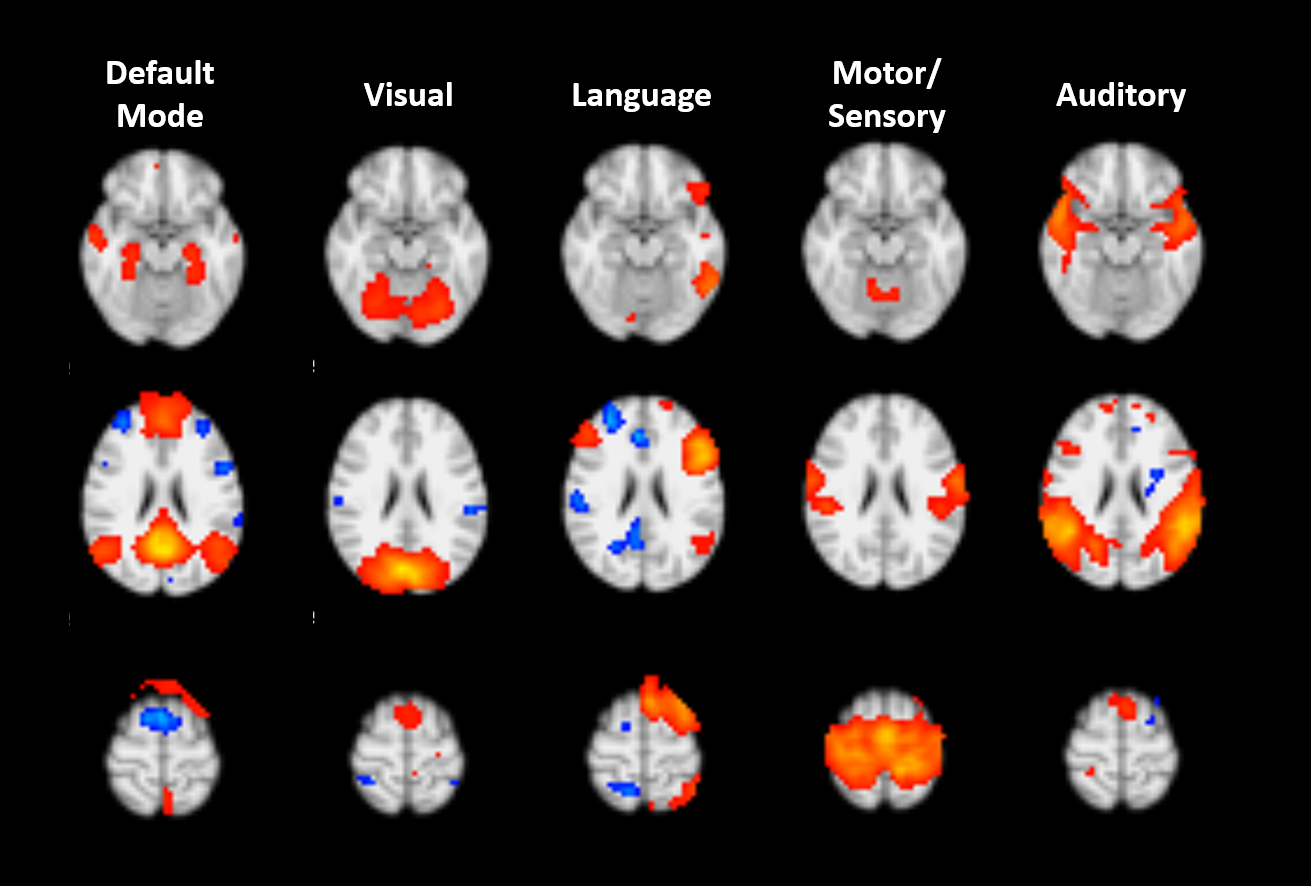
\includegraphics[width=12cm]{Ch1_ICA}
    \caption[Examples of resting-state networks.]{Examples of resting-state networks derived from 16 adult subjects at rest. fMRI data were decomposed into 21 independent components and thresholded at p \textgreater 0.7.} 
\end{figure}

Beyond simply identifying these networks, scientists have used graph theory to analyze how the brain areas that make up these networks act in terms of the entire system of brain networks (sometimes called the connectome). In graph theory, each brain area is a single "node" in the larger brain network and temporal correlations with other nodes are "edges". In RS-fMRI, similar cortical areas (e.g. Brodmann areas) are typically assigned to to be nodes. In some cases, the entire brain is input into the analysis, whereas others use a more targeted, seed-based approach \cite{Vogel2010}.  Edges are often weighted, meaning areas that are more highly correlated carry a greater connectivity value. Next, an algorithm is applied to the matrix of correlations to distinguish sets of nodes that are more highly connected to each other than to other areas of the brain. Finally, first- and second-level properties of the networks, are derived.

The decision of which regions to include as nodes is critical. Typically, one of several approaches has been used to identify nodes: anatomical parcellations based on an atlas \cite{Supekar2008, Liu2008, Lynall2010}; individual voxels \cite{Fair2007}; functional ROIs from either a priori hypotheses or task-based activation \cite{VandenHeuvel2010}; or an algorithm that parcellates the brain independent of function or anatomy \cite{Goni2014}.  Differences in these methods can affect the RSNs identified. At high resolutions (e.g. voxel-level correlations), there is a greater chance of spurious correlations causing noise in the data; at lower resolutions, the timeseries for a region may blend multiple functional regions, creating a composite that does not truly reflect any of the underlying areas. 

Graph theory provides several metrics for consideration, of which we discuss three: \textit{node degree} is the number of connections a single node has \cite{Sporns2013}. Nodes with higher degrees are thought to communicate with a greater number of nodes than others; networks with a higher average degree are thought to be more densely connected. \textit{Path length} is the minimum number of nodes that must be passed to connect one node to any other. A completely random network will have a relatively low path length; a completely regular one will have a high path length. Finally, the \textit{participation coefficient} is the degree to which a node participates in networks other than its primary one. These properties have been used to find a number of interesting things about the brain. 

Developmentally, RSNs exhibit increasing functional correlation across the lifespan \cite{Kesler2013, Uddin2010}. Properties of these RSNs, including density of connections, along with their locations and changes with development is of primary interest  \cite{Cole2014, Dosenbach2007, Fair2009}. RSNs in children are more greatly constrained by proximity than in adults but are functionally organized: visual system regions, for example, form their own community, as do auditory regions and executive control regions \cite{Seeley2007}. Several studies report that the brain takes on a modular structure, consisting of many densely intra-connected networks \cite{Bullmore2009, Fair2009, Supekar2009, Dosenbach2007}. These modules are connected to each other by a smaller number of regions, dubbed "rich clubs" or "hubs", that may facilitate the passage of information from one module to another \cite{Power2013, Bullmore2012}. 

\begin{figure}[t]
    \centering
    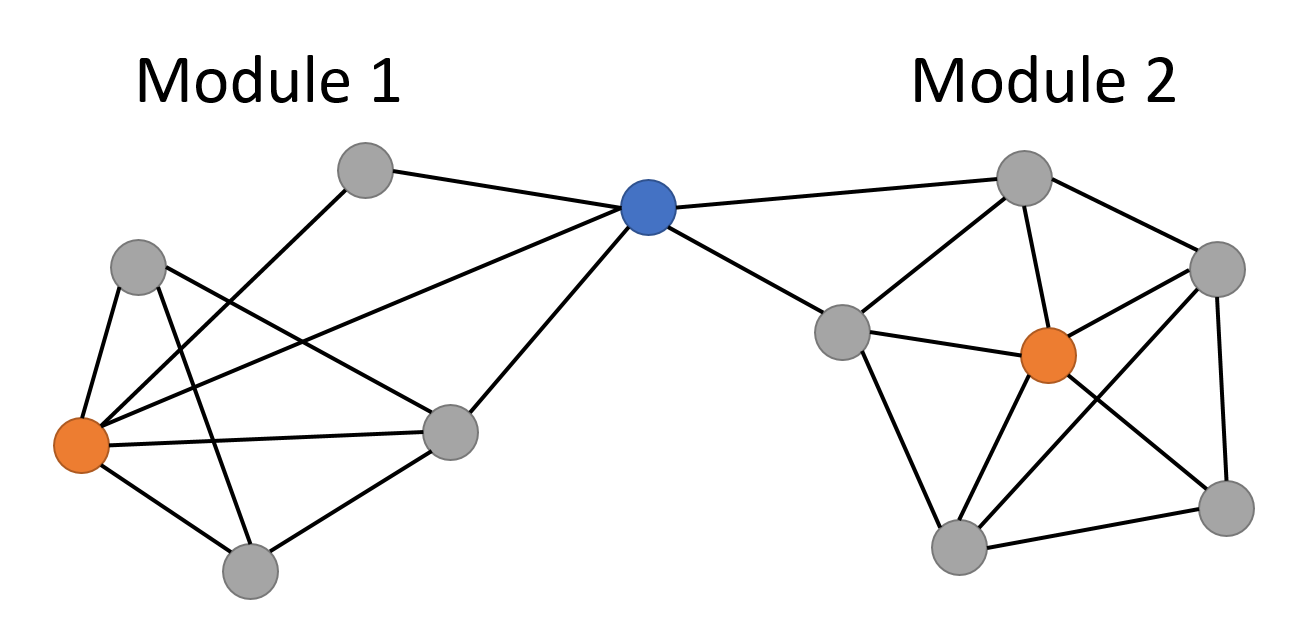
\includegraphics[width=14cm]{Ch1_GraphSchema.png}
    \caption[Schematic for a network with two modules.]{Schematic for a network with two modules. The blue node is a hub region critical for connecting modules 1 and 2. The orange nodes have the highest degree of all nodes.}
\end{figure}

\subsection{General applications of graph theory}

These findings have informed our understanding of the brain's large-scale organization. Rather than having a set of tracts that connect all regions, these findings suggest the brain is organized complexly but efficiently in a "small-world" architecture. This has emphasis on the importance of certain regions to fulfilling cognitive functions: in one study with lesioned patients, Petersen et al. predicted how severe a lesion would be based on its proximity to these hub regions \cite{Warren2014}. They found that lesions on areas that were not densely connected showed less extended impairments than regions which were highly inter-connected in RS-fMRI. Other psychiatric disorders have found disruptions in network properties. Lord et al. found that while whole-brain metrics of modularity were similar across individuals with depression and , RSNs "reorganized" in individuals with depression \cite{Lord2012}. Thus network properties may be important for explaining individual differences in neuropsychiatric disorders or cognitive skill, such as comprehension. 

Relatively few studies have been done relating network methods to reading ability. Despite the changes in connectivity between areas, reading-related regions such as the fusiform gyrus, angular gyrus and inferior frontal gyrus, do not create one distinct RSN, but are members of separate, more primary RSNs \cite{Vogel2013}. Finn et al. compared graph theory metrics of dyslexic and non-impaired readers using graph metrics \cite{Finn2014}. Dyslexic readers showed divergent activity in visual association and prefrontal attention areas as well as increased right-hemisphere connectivity. Differences were persistent across both adult and children readers, suggesting that network metrics are relevant for reading. Another study investigating how graph theory metrics changed in response to sentence-level processing showed that network properties were relatively stable \cite{Ye2012}. Participants were asked to silently read a sentence that had either a semantically congruent or incongruent ending. Furthermore, metrics showed that subcortical processing (basal ganglia to supplementary motor area) was stronger in response to incongruent versus congruent endings. 

According to the view of interactive specialization, an integrative ability like reading comprehension would be more highly connected. The multi-RSN robustness, or the how well-maintained the network is after deletion of a node, will measure how strongly inter-connected the RSNs of interest are to each other \cite{Bullmore2009}. An important consequence of these hypotheses is that, if there is a biological substrate underlying RC, we may have another window into predicting how well a child will continue to develop as a reader, especially during the periods of rapid development in primary school.

One promising area of application is that of prediction. Machine learning techniques such as multivariate pattern analysis have been used to classify individuals with developmental and neuropsychiatric disorders before, including individuals with dyslexia \cite{Ecker2010, Hoeft2011, Wee2014, Hoeft2007, Ingalhalikar2014}, autism and depression \cite{Lord2012}.  These techniques can incorporate multiple sources of information, such as network properties, to build the optimal model for predicting whether a dataset belongs in one group relative to another \cite{Pereira2009}. This has been done with anatomical and functional data \cite{Hoeft2007, Hoeft2007b}. Network properties may be even more likely to contain information about an individual's likelihood of succeeding in school than other metrics.

However, the neurobiological basis for these RSN properties is still under investigation. While these connections do appear to be plastic and mediated by experience, they are not necessarily caused by new synapses. Several studies using diffusion-weighted MRI (DW-MRI) suggest that functional connectivity represents more than simply direct synaptic connections. Diffusion-weighted MRI (DWI) uses water movement to model the white matter tracts within the brain. At high resolutions, it provides a coarse approximation of the human connectome -- the total connections in the human brain \cite{Sporns2005}. Honey et al. investigated whether functional connectivity can be predicted from structural connectivity \cite{Honey2009}. Five subjects underwent DW-MRI and RS-fMRI scans, and brains were parcellated at both a high resolution (998 cortical regions) and low resolution (66 cortical regions). They found that, while structurally connected areas are typically functionally connected as well, the inverse is not true. Areas that were closer together were also more highly functionally connected, possibly due to structural cortico-cortical projections. 

More work, including longitudinal studies, certainly needs to be done to understand the complex processes. One of the outstanding questions in the field, though, is what (and even whether) these properties have a neural or psychological basis. While it is likely that RSNs reflect a long history of co-activation between brain areas \cite{Cohen2008, Fair2008}, it is less clear what individual differences in a specific metric might mean.


\subsection{Distribution of resting-state networks across reading areas}
Reading-related regions were selected on the basis of the Neurosynth meta-analytical database \cite{Yarkoni2011}, comprising 11,406 studies as of October 31, 2017. NeuroSynth aggregates brain activation data from thousands of studies to return activation likelihood maps based on search terms. The database was queried for "reading", yielding 427 studies. NeuroSynth provides two meta-analysic activation maps, one using forward-inference and the other using reverse-inference. The forward-inference map creates a map of brain areas associated with reading-related papers; the reverse-inference map returns the set of brain areas most likely to be active only in reading-related papers. The reverse-inference map thus de-weights domain-general functional areas and is more representative of reading-specific areas than the forward-inference map. Because domain-general processes are fundamental to skilled reading (especially comprehension), our primary interest was in the forward-inference map, but both maps were examined. 

The 7-network cortical parcellation from Yeo and colleagues (2011) was used to represent canonical RSNs \cite{Yeo2011}. On the basis of resting-state fMRI data from 1000 subjects, this atlas identifies the following RSNs: visual, somatomotor/auditory, limbic, ventral attention, dorsal attention, default mode, and fronto-parietal. The "Liberally Masked" volumetric data was downloaded in MNI152 space and co-registered to the NeuroSynth data. For each inference map, the percentage of activation falling into each RSN (cm\textsuperscript{3}) was calculated to provide a distribution across each RSN.

A comparison of the NeuroSynth "reading" activations to the 7-network parcellation from Yeo and colleagues shows that reading is widely distributed across resting-state networks (Fig. 1). In the forward-inference map, the visual and somatomotor-auditory RSNs consituted about one quarter of the NeuroSynth activations (17.5 and 8.2 percent, respectively), while attention networks combined to make up 37 percent. The fronto-parietal (19.3 percent) and default mode (17.8 percent) networks were were also highly represented. The limbic network was the only RSN which did not meaningfully overlap with the reading network. Compared to the baseline distribution of the Yeo parcellation, the visual, dorsal attention, ventral attention and fronto-parietal networks consituted a larger portion of the activation; the limbic, somatomotor and default mode had smaller shares (Table 2). 

The NeuroSynth reverse-inference map was smaller than the forward-inference map by 28.7 percent and was restricted to areas more specific to reading. In particular, there was a higher involvement of the visual (+3.9 percent) and default mode network (+11.8 percent) compared to the forward-inference map. On the other hand, networks supporting domain-general functions (dorsal attention, ventral attention, fronto-parietal) were relatively less present (-3.4, -6.7 and -6.0 percent, respectively). Representation of the somatomotor-auditory and limbic network involvement was mostly unchanged.

\begin{figure}
\centering
\includegraphics[width=5in]{Ch1_YeoReading.png}
    \caption[Reading areas are distributed across many resting-state networks.]{Reading areas are distributed across many resting-state networks. On the left is the volumetric breakdown of the "reading" network, pulled from a NeuroSynth automated meta-analysis (forward-inference: $p < 0.01$, FDR-corrected) \cite{Yarkoni2011}, according to the 7-network cortical parcellation from Yeo and colleagues \cite{Yeo2011}. On the right is a surface plot of the same data. Reading areas are well-distributed across different networks and load highly onto attention and executive networks. Several important reading areas, including the inferior frontal gyrus and temporo-parietal junction, sit at points where multiple networks converge, i.e. likely hub areas.}
    \label{fig:texlogo}
\end{figure}



\subsection{RSN contributions to reading}
A tremendous amount of research has been done investigating "lower-level" reading skills, such as phonological processing and symbol-phoneme mapping. And while reading researchers in the past decade have begun to acknowledge the contributions of domain-general skills (e.g. attention, working memory, planning and organizing) to reading, it remains a secondary concern in much neuroimaging literature. (We caution that this is not the case for all language research, but specifically reading.) However, attention and executive networks constitute more than half of the activity observed in reading tasks (Fig. 1). Below is a brief survey of intersections between these RSNs and reading theory which may provide good candidate hypotheses for investigation.

\subsubsection{Attention networks drive and suppress sensory integration} 
Attention underlies skilled reading at all levels: it is critical for identifying only the salient words in a large block of text, for suppressing environmental distractions and for maintaining focus for extended periods of time. In a common framework for attention, the dorsal and ventral attention networks (DAN and VAN) play collaborative roles for guiding focus. (The "salience" network, is sometimes differentiated from the VAN. For a detailed summary, see \cite{...}.) Simplistically, the DAN exerts top-down control of sensory processes to keep a person on task, while the VAN detects salient or unexpected stimuli, acting as a "circuit breaker" to help reorient the person \cite{Corbetta2002, Vossel2014}. This relationship may be impaired in individuals with dyslexia that have "sluggish attention shifting" attention between visual and auditory modality \cite{Harrar2014}. Slow or inadequately rapid attention-shifting could undermine fluent reading by causing temporal-spatial misalignment in processing, e.g. letter sequence and arrangement \cite{Lallier2009}. This deficit in attentional shifting is argued to further characterize dyslexic readers’ rapid temporal and low spatial frequency processing (e.g., \cite{Ingelhem2001, Witton1998}). Asynchronicity within this system is argued to be characteristic of dyslexia \cite{Vidyasagar2009, Lallier2009, Ingelhem2001}). Online interaction between the DAN and VAN during reading may thus index some of the attentional switching problems that are apparent in dyslexia. 


\subsubsection{The visual word form area is part of the DAN} 
The visual word form area (VWFA) performs an important role in orthographic processing, and activity in the VWFA is sensitive to letter size, font and other orthographic attributes \cite{References from Vogel2011}. It's alleged specificity to language has been a source of controversy over the past decade \cite{...}, however, and several have argued that its importance in reading is directly linked to its membership in the DAN \cite{Vogel2014}. During reading, the DAN supports appropriate textual features or chunks and suppressing distracting information elsewhere \cite{Corbetta2002}. At issue in the debate is how general or specific visual attention deficits are in dyslexia \cite{Vogel2011}. Decreased activation in the pVWFA to text relative to typically developing participants has been reported in many studies of dyslexia \cite{...}, but these differences could be due to more generalizable visuo-spatial deficits. For example, fluent reading requires accurate and precise eye movements \cite{Rayner1998}, and a key node in the DAN is the "frontal eye fields" which help coordinate saccadic activity \cite{Petit1997,Connolly2000}. In fact, a number of studies report deficits in visual attention in children with RD (for a review, see Vidyasagar and Pammer 2010). Children with RD deficits in processing of consonant strings \cite{Pammer2004} and in matching symbol strings \cite{LassusSangosse2008}. Koyama et al. (2013) found that children with a historical diagnosis of dyslexia had persistant de-coupling of the dorsal attention network compared to typical readers regardless of remediation status \cite{Koyama2013}. Vogel et al. (2012) found that reading ability in typical children and adults (including decoding and passage comprehension ability) predicted increased correlations between the visual word form area and the dorsal attention network \cite{Vogel2012}. Whatever the true cause, it is clear that the DAN provides critical support for reading, above and beyond simply processing stimuli.
% Get at the deeper questions... not just orthographic processing, bu tpassing along information


\subsubsection{Executive networks coordinate other cognitive processes} 
Executive functions play an important role in predicting reading outcomes, especially when considering comprehension \cite{Cutting2008}. Although the variety of cognitive processes that fall under EF construct do not map cleanly onto a single brain region or network, they are closely associated to the "central executive" system. This in turn is mapped on to the fronto-parietal network (FPN) (and sometimes the cingulo-opercular network) \cite{Fedorenko2013, Cocchi2013}. Unlike many other RSNs, the FPN has components which are not neighboring, spanning portions of the frontal and parietal lobes \cite{Yeo2011}. Interestingly, the FPN has recently been hypothesized to act as a neural mediator of other brain systems \cite{Mennon2010, Cole2014} by using wide-spread cortical connections to facilitate efficient processing of other networks, and in particular assist when areas are not functioning adequately. According to this coordinator model of the FPN, greater symptoms of dyslexia may correspond with reduced functional and structural integrity of the FPN. For instance, Norton et al. compared brain activation and connectivity in DYS reader sub-types, including readers with rapid naming deficits only, phonological awareness deficits only, and double deficits (i.e. poor rapid naming and phonological awareness) \cite{Norton2014}. They found graded de-activation and de-coupling of the FPN during a word rhyme judgment task, with the most severe deficit sub-group (double deficit) showing the greatest FPN de-activations and internal de-coupling. In the only functional connectomics paper on young readers with dyslexia, Finn et al. (2013) examined whole-brain connectivity during a word/non-word rhyming task, and found that children (and adults) with dyslexia showed de-coupling of frontoparietal areas \cite{Finn2013}. 


\subsubsection{Executive networks may support intervention response}
In addition to coordinating other RSNs, the FPN may play a role in supporting systems \cite{Cole2015}. Horowtiz-Kraus et al. (2015) examined resting state functional connectivity in young readers with and without dyslexia who had undergone a reading intervention \cite{HorowitzKraus2015}. They found that after intervention, readers with dyslexia had improved connectivity between a visual component and bilateral regions in the FPN (notably, as in many studies on reading, the latter component was not identified as an FPN component, but instead discussed as a language network). Furthermore, Koyama et al. (2013) examined resting state connectivity in dyslexic readers with variable remediation status, and found that children with a historical diagnosis of dyslexia had persistent de-coupling of frontoparietal areas compared to typical readers, regardless of remediation status \cite{Koyama2013}. Additionally, in the first reading study to examine functional interactions across networks, Aboud et al. (under review) found that, prior to intervention, readers who were responsive to the intervention mediated reading network connectivity via a key node in the FPN, the dorsolateral prefrontal cortex (dlPFC) \cite{Aboud2017_NF}. These findings support the hypothesis that executive areas in the FPN might act to facilitate the functional integrity of other systems necessary for reading.


\subsubsection{Default mode network engagement and disengagement} 
The DMN is a network of inter-connected regions (including medial prefrontal cortex, bilateral inferior parietal lobules, and posterior cingulate cortex) \cite{Shulman1997}. Since its original discovery, the DMN has since been found to support a wide range of cognitive processes often classified under internal mentation \cite{Buckner2008}, including theory of mind, narrative processing, and autobiographical recall \cite{AbdulSabur2014}. The DMN exhibits a large amount of overlap with traditional reading areas, including major comprehension-related regions such as the angular gyrus and anterior temporal pole. However, the DMN also has antagonistic relationship with "task-positive" attention networks such as the FPN, where the activation of one network necessarily comes at the suppression of the other, and this relationship appears to be important for performance on a variety of cognitive processes \cite{Fox2005, Keller2015}. Consequently, appropriate FPN involvement may be best achieved by suppression of the DMN. Several studies point to over-involvement of the DMN in readers with dyslexia, including higher internal correlations of the DMN during reading \cite{Finn2013} and greater correlations between the DMN and reading areas during reading and at rest \cite{Schurz2015}. Given that activity in both the FPN and DMN are critical for reading comprehension, understanding the dynamics of this relationship could be particularly illuminating.



\subsection{Mapping dyslexia abnormalities onto hub areas}
Two decades of neuroimaging research have allowed a relative consensus to form as to which brain regions are commonly dysfunctional in dyslexia. To determine whether there was any pattern related to network architecture in these areas, we gathered all clusters from three meta-analyses comparing fMRI activation for individuals with dyslexia to typical readers \cite{Maisog2008, Richlan2009, Paulesu2014}. All areas that showed atypical activation in dyslexia (either greater or less activity) were included. When a cluster was large, all reported local maxima were included. 

To get measures of hubness across the brain, we used data from a connectomics study by Power and colleagues (2013) \cite{Power2013}. That study reports the \textit{participation coefficient} for each of the 264 nodes previously described. The participation coefficient reflects the diversity of a node's connectivity to different RSNs, where a higher value indicates that the node is correlated with many different RSNs. Activations from the dyslexia meta-analyses were then mapped to the geometrically closest node from this dataset, resulting in a small set of dyslexia-related nodes and a larger, unaffected set.

The distribution of participation coefficients across the 264 nodes was non-normal, with a large group of areas having low participation coefficients (i.e. affiliated with few RSNs) and a smaller hub-like group. Therefore, a Wilcoxon rank-sum test was performed on the participation coefficients for the two groups, which tests for the equivalence of two distributions in a non-parametric fashion.

Across the three meta-analyses, 32 of the 264 nodes showed abnormal functioning in dyslexia. Figure 3 shows the node-by-node distribution of participation coefficients for the entire set. The median participation coefficient for unaffected nodes was 1.47; for dyslexia-related nodes it was 3.28. A Wilcoxon rank-sum test between the dyslexia and unaffected nodes showed that dyslexia affects brain areas with higher participation coefficients than would otherwise be expected ($U = 4946.0$, $p$ \textless $0.001$). 

\begin{figure}[h!]
\centering
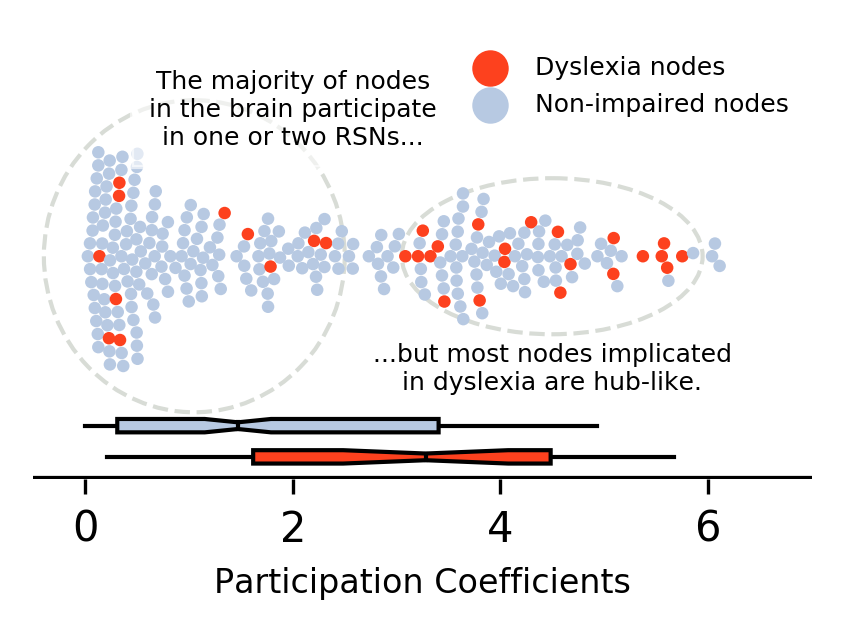
\includegraphics[width=5in]{Ch1_DyslexiaHubs.png}
    \caption[Dyslexia disproportionately impacts hub areas.]{Dyslexia disproportionately impacts hub areas. Among the brain areas examined in Power and colleagues (2013), nodes implicated in dyslexia have higher participation coefficients (32 nodes) compared to the rest of the brain (232 nodes).}
\label{fig:texlogo}
\end{figure}


\subsection{How the brain reconfigures (Cohen + Esposito)}
A critical feature of the human brain that gives rise to complex cognition is its ability to reconfigure its network structure dynamically and adaptively in response to the environment. Existing research probing task-related reconfiguration of brain network structure has con-cluded that, although there are many similarities in network structure during an intrinsic, resting state and during the performance of a variety of cognitive tasks, there are meaningful differences as well. In this study, we related intrinsic, resting state network organization to reconfigured network organization during the performance of two tasks: a sequence tapping task, which is thought to probe motor execution and likely engages a single brain network, and an n-back task, which is thought to probe working memory and likely requires coordination across multiple networks. We implemented graph theoretical analyses using functional connectivity data from fMRI scans to calculate whole-brain measures of network organization in healthy young adults. We focused on quantifying measures of network segregation (modularity, system segregation, local efficiency, number of provincial hub nodes) and measures of network integration (global efficiency, number of connector hub nodes). Using these measures, we found converging evidence that local, within-network communication is critical for motor execution, whereas integrative, between-network communication is critical for working memory. These results confirm that the human brain has the remarkable ability to reconfigure its large-scale organization dynamically in response to current cognitive demands and that interpreting reconfiguration in terms of network segregation and integration may shed light on the optimal network structures underlying successful cognition.
\chapter{Reorganization of network architecture during reading and listening}

\epigraph{Reading is parasitic on language... [It] is seen not as a parallel activity in the visual mode to speech perception in the auditory mode: there are differences... [that] can be explained only if we regard reading as a deliberately acquired, language-based skill, dependent up on the speaker-hearer's awareness of certain aspects of primary linguistic activity.}{I. Mattingly, 1972 \cite{Mattingly1972}}

\section{Motivation}

In the first chapter, I established that reading utilizes a variety of cognitive skills whose neural substrates are distributed throughout the brain. But being able to comprehend speech is a pre-requisite to reading, and it is similarly complex. It begs the question: in what ways is reading unique from listening?

The most widely-held view is that reading and listening share the same core linguistic processes and differ primarily in the sensory processes that feed into supra-model linguistic systems \cite{Mattingly1972, Price2012}. One popular model, the \textit{Simple View of Reading} makes this testable by stating that reading comprehension is the product of listening comprehension and decoding skills \cite{Gough1988}. This view has received support from large behavioral studies \cite{...} and neuroimaging investigations: many of the literacy-related changesare linked to visual or phonological systems, areas not directly related to semantic or comprehension processes \cite{Schlaggar2006, Dahaene2015}. 

Neuroimaging studies support a model in which inputs from auditory or visual domains are fed up into higher-order association areas that sequence, encode articulatory plans, and extract semantic information \cite{Price2012}. These processes localize onto the similar areas regardless of language and writing system \cite{Rueckl2016}, and may even extend to inputs from somatosensory domains \cite{Xu2005, Sood2015}. This supra-modal language core is largely left-lateralized and centers on the inferior frontal gyrus, anterior and posterior middle temporal gyrus and the angular gyrus. Neuroanatomical models of language, shown in Fig. \ref{ch2-price-language-models}, illustrate that language is distributed throughout much of the brain. 

\begin{figure}[tp]
	\centering
	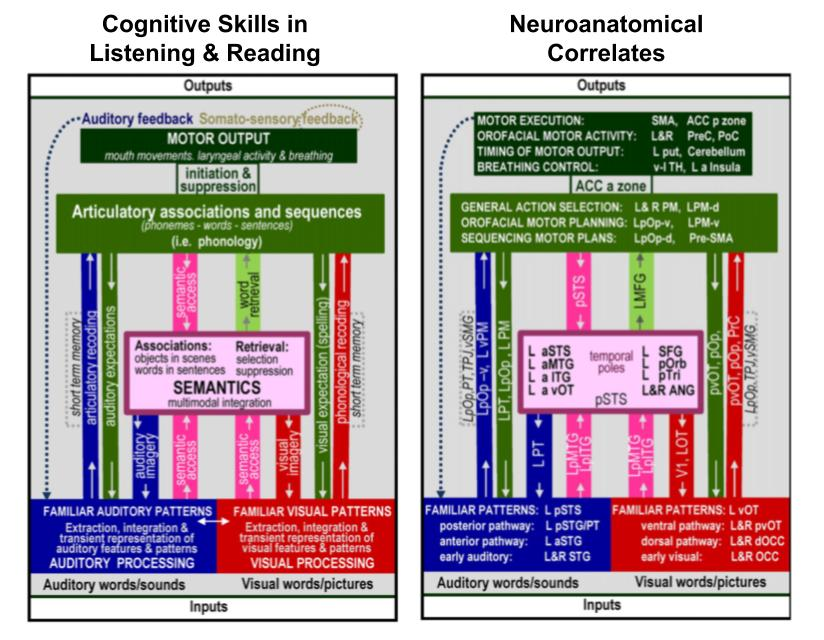
\includegraphics[width=5in]{images/ch2-price-language-models.jpg}
	\caption[Schematics of skills and brain areas used in reading.]{Models of reading typically focus on a common linguistic core that is responsible for comprehension and production of language. In this model, differences in modality affect input pathways to this core.}
	\label{fig:ch2-price-language-models}
\end{figure}

However, there is evidence that comprehending written and spoken language are not equivalent. There is a subset of students who, despite adequate word decoding skills and vocabulary skills, struggle with reading comprehension\citep{Nation2010, Spencer2011}. From a neurobiological perspective, expected differences in primary visual (for reading) and primary auditory (for listening) represent the different input systems, with ventral occipito-temporal systems also activating \cite{Jobard2007}. However, differences in core language systems are also observed: additional activation in left posterior temporal and parietal areas in reading modality (Constable et al., 2015), as well increased bi-laterality especially in children \cite{Berl2010}. 

Most current cognitive models suggest that language comprehension requires the construction of a mental representation includes textual information and associated background knowledge, connected by some conscious and some unconscious executive processes \cite{Kendou2014}. The parallel model shown in Fig. \ref{fig:ch2-price-language-models} is linear: it moves from sensation to action. During comprehension, however, the relationship between areas is dynamic and constantly being re-evaluated. The roles of attention and executive systems are likely to play an important role. Thus, while there may be a core set of systems for manipulating and extracting meaning from language, it is likely that differences in modality would modulate these processes.

In this study, I pursue three hypothesized ways reading might differ from listening. These are not exclusive; one or more of them may be true. The overarching aim is to test whether reading is \textit{simply} listening skills

\begin{itemize}
	\item Reading will reduce the modularity within the sensory system of interest. That is, visual areas will become less internally connected during reading, while auditory areas will be less internally connected during listening.
	\item Reading will make greater demands on attention and executive systems than listening. That is, areas in the frontal and attention systems will be activated to a greater degree during reading than listening.
	\item Reading will induce greater cross-network connectivity than in listening. 
\end{itemize}

Such a line of investigation is particularly valuable in the context of developing readers, who are mapping visual systems onto existing language circuitry: identifying differences between reading and listening comprehension may elucidate which systems uniquely support reading comprehension. In this study, I use graph theory and functional data from listening and reading tasks to describe the local and global reorganization of the brain in children aged 9 to 11.

First, we validate modularity and participation coefficient metrics using univariate data, and test that language induces greater global integration, especially in higher-order networks (executive + default mode) compared to resting and attention baselines. Second, we test three hypotheses about how interactions between brain networks might differ from speech. Finally, we investigate whether these interactions change with experience, testing whether the reading and listening systems "merge" into a unified system or whether differences between reading and listening persist across development.


\section{Methods}

The following methods detail the current study's protocol and analytical approach. Many of these methods will be used in future studies and are explained in detail here. 

\subsection{Participants}

Participants for the first study were drawn from the fourth wave of a larger, longitudinal study investigating the neurobiological bases of reading comprehension. 50 children completed scans for the current study, and a subset of these met the motion and attention thresholds described below. See Table \ref{table:ch2-participants} for demographics. 

All participants were native English speakers with normal hearing and normal or corrected vision, and no history of major psychiatric illness or traumatic brain injury/epilepsy. Subjects had no history of a developmental disability or contra-indication to MRI.  Each participant gave written consent at the beginning of the study, with procedures carried out in accordance with Vanderbilt University’s Institutional Review Board.

\begin{table}
	\scriptsize
	\renewcommand{\tabcolsep}{0.09cm}
	\centering
	\begin{tabular}{lc}
\toprule 
Measure & Subjects \\ 
\midrule 
No. Participants				& 42 \\ 
No. Scan Runs					& 164 \\ 
Gender  						& 25 F \\ 
Age at Scan 					& 10.5 (0.3)  \\ 
WASI Full-Scale IQ  			& 111.0 (16.2) \\ 
TOWRE - Total Word Efficiency 	& 104.6 (18.5) \\ 
\bottomrule 
\end{tabular}
	\caption[Participant demographics for Study 1.]
	\label{table:ch2-participants}
\end{table}


\subsection{Functional MRI Task}

We designed an fMRI task in which participants either read or listened to a passage of text. The passage was split into two paragraphs and interspersed with a simple attention task. At the end of the task, there was an approximately three minute long resting-state block. Across runs, conditions were presented in the same order, although durations varied slightly. Condition order was: comprehension block (paragraph 1), sensory baseline (set 1), comprehension block (paragraph 2), sensory baseline, and resting baseline. See Fig. \ref{fig:ch2-task-design} for a schematic.

\begin{figure}[tp]
	\centering
	\includegraphics[width=5in]{images/ch2-eprime-recall.png}
	\caption[Schematic of the reading comprehension task.]
	\label{fig:ch2-task-design}
\end{figure}

To create a more naturalistic reading experience than single word presentation \citep{Rayner1986}, passages were presented in syntactic phrases ranging from 1-7 words in length. The interval between each stimulus was jittered to allow for event-related analyses (range: 275 – 4000 ms), although these effects were not examined here.

The sensory baseline condition was altered according to modality. For the reading runs, three non-alphanumeric symbols were displayed horizontally (two types), and their presentation time was matched to the passage phrases. Spacing between symbols was randomly alternated to replicate the variable phrase lengths in the passage condition. For the listening runs, three tones (two frequencies) were played in sequence, with a new set of tones beginning at the same intervals as the corresponding passage presentation. 

To monitor attention, 4 to 8 percent of the stimuli within each passage or attention block were randomly repeated on two consecutive screens.  Participants pressed a button with their right thumb when they detected a repeated phrase, symbol or tone configuration. Additionally, at the conclusion of each passage, a picture was presented on the screen, and subjects were asked to identify whether the picture had any relationship to the passage (e.g., a picture of a mushroom for a passage about fungi). 

To assess performance, we analyzed three measures: in-scanner attention, in-scanner comprehension, and post-scan recall. To assess attention, we calculated the $D`$ statistic ($Z(true\ positive) - Z(false\ positive)$) for the "repeated stimulus" task. The in-scanner comprehension measure was the number (0,1,2) of questions correclty answered. To assess recall, each child was asked to recite as much of the passage as they could remember, and their answers were mapped to actual phrases present in the chapter. Individual scan runs with a $D`$ value less than 2 were excluded from analysis.

In total, there were 4 passages (2 listening, 2 reading), each leveled to a 3\textsuperscript{rd} grade difficulty and balanced word measures such as concreteness and cohesiveness.  All subjects were trained on the task in a mock scanner prior to the actual scan. 


\subsection{MRI acquisition}

Imaging was performed on a Philips Achieva 3T MR scanner with a 32-channel head coil. Functional images were acquired using a gradient echo planar imaging sequence with 40 (3 mm thick) slices with no gap. Each run of the task (up to four) consisted of 250 volumes. Slices were parallel to the anterior-posterior commissure plane. Imaging parameters for functional images included: TE = 30 ms; FOV = 240 x 240 x 120 mm\textsuperscript{3}; flip angle = 75\degree; TR = 2200 ms; and 3 mm\textsuperscript{3} isotropic voxels.

\subsection{Activation analyses}

Whole-brain fMRI analyses were performed using tools from the FMRIB Software Library (version 5.0.9). For each session, the following pre-processing steps were performed:  slice-time correction, motion correction to the initial fMRI volume, high-pass filtering at 0.08 Hz, boundary-based registration to the subject's structural image, and normalization to 2 mm MNI 152 standard space. To mitigate the effects of motion on our analyses, we regressed out 6 continuous motion parameters and scrubbed out outlier volumes. We defined an outlier volume as any in which the root-mean-square framewise displacement exceeded 0.7 mm. Because head motion can be a major confound for connectivity analyses, we removed scan runs where more than 10 percent of the fMRI volumes were outliers.

All task conditions were convolved with the double-gamma hemodynamic response function to generate design matrices for each fMRI run. Two first-level contrasts were of interest: the main effect of passage comprehension (“PASS vs. REST”), and the contrast of passage comprehension vs. the sensory baseline ("pass vs. attn."). Repeated stimuli and the picture comprehension task were modelled out.

Modality effects (Shared Effect of Listening and Reading, Contrast of Listening and Reading) were estimated at the subject-level using fixed effects analysis. These were carried over into group-level analyses using non-parametric methods implemented in FSL’s \textit{randomise} tool with threshold-free cluster enhancement. For each group-level analysis, we performed 10,000 permutations and report results with \textit{p} \textless 0.05. 

\subsection{Connectivity analyses}

To investigate whole-brain patterns of connectivity without biasing our results towards our task, we selected 264 nodes \textit{a priori} whose connectivity properties have been extensively analyzed \citep{Power2011}. This node set samples the entire brain and are involved in a diversity of cognitive tasks. Each node was assigned to one of 13 RSNs based on previous literature \citep{Power2013}. Approximately 10 percent of the nodes fell did not have a stable assignment in the original paper; for the present analyses, these nodes were excluded from graph theory calculations. A description of the 13 networks, their size, and their overlap with the 2011 Yeo parcellation is provided in \ref{table:ch2-power-nodes}. 

\begin{table}
	\scriptsize
	\renewcommand{\tabcolsep}{0.09cm}
	\centering
	\begin{tabular}{lcc}
\toprule 
Suggested RSN & Abbreviation & Nodes \\ 
\midrule 
\textit{Sensory} & & \\
	\hspace{3pt}Auditory  			&  AUD & 13 \\ 
	\hspace{3pt}Somatomotor (Hand)	&  SOH & 30 \\
	\hspace{3pt}Somatomotor (Mouth)	&  SOM & 5 \\
	\hspace{3pt}Visual	 			&  VIS & 31 \\ 
\textit{Attention} & & \\
	\hspace{3pt}Dorsal attention  	&  DAN & 11	\\ 
	\hspace{3pt}Salience		  	&  SAL & 18 \\ 
	\hspace{3pt}Ventral attention  	&  VAN & 9 \\ 
\textit{Executive / Associative} & & \\
	\hspace{3pt}Cingulo-opercular 	& CON & 14 \\ 
	\hspace{3pt}Default mode		& DMN & 58 \\
	\hspace{3pt}Fronto-parietal  	& FPN & 25 \\ 
	\hspace{3pt}Memory retrieval	& MEM & 5 \\
\textit{Other} & & \\
	\hspace{3pt}Cerebellar			& CER & 4  \\
	\hspace{3pt}Subcortical			& SUB & 13 \\
	\hspace{3pt}Not assigned 		& UNC & 28 \\ 
\bottomrule 
\end{tabular}
	\caption{Networks used in connectivity analyses.}
	\label{table:ch2-power-nodes}
\end{table}

Network estimation was performed in the \textit{Conn: Functional Connectivity Toolbox} (version 17f) \citep{Nieto-castanon}. For each scan run, the BOLD activity at each node was denoised using the anatomical CompCorr method, which regresses out background noise from white matter and cerebrospinal fluid tissue. We also regressed out 12 continuous measures of motion were also included, all outlier timepoints, and the effect of all task conditions ("pass", "attn", "rest"). The timeseries was then high-pass filtered at 0.01 Hz.

Whole-brain connectomes for each condition were created by estimating the functional connectivity between each node using a weighted general linear model. For connection-level analyses, these values were compared directly across subjects and conditions. For graph theory analyses, the array of all node connections was thresholded to keep the top 5 percent of connections, resulting in a much sparser representation. This threshold was also tested at ranges from 2 percent to 10 percent.

The metrics of interest were network \textit{modularity} and \textit{participation coefficient}. Modularity is high in networks where nodes within the same RSN are highly connected to each other but not elsewhere. The participation coefficient, on the other hand, is high when many nodes are connected to several different RSNs. Both of these metrics relate to the integration of information between RSNs. These properties, and their changes within our task, were investigated at the level of connectomes, RSNs and nodes. 


\section{Results}

\subsection{Behavioral results}

35 subjects (116 scan runs) met the attention and motion criteria to be included in the analysis. (17 subjects and 87 individual scan runs were filtered out.) Attention and comprehension measures were not related to modality of stimulus presentation (see Figs. \ref{fig:ch2-eprime-recall} and \ref{fig:ch2-eprime-comprehension}). There was no difference in median FDRMS between scan modalities (paired t-test, $t = 1.09$, $p = 0.279$).  

\begin{figure}[tp]
	\centering
	\includegraphics[width=5in]{ch2-eprime-recall}
    \caption[Out-of-scanner pasage recall was unrelated to modality.]{}
	\label{fig:ch2-eprime-recall}
\end{figure}

\begin{figure}[tp]
	\centering
	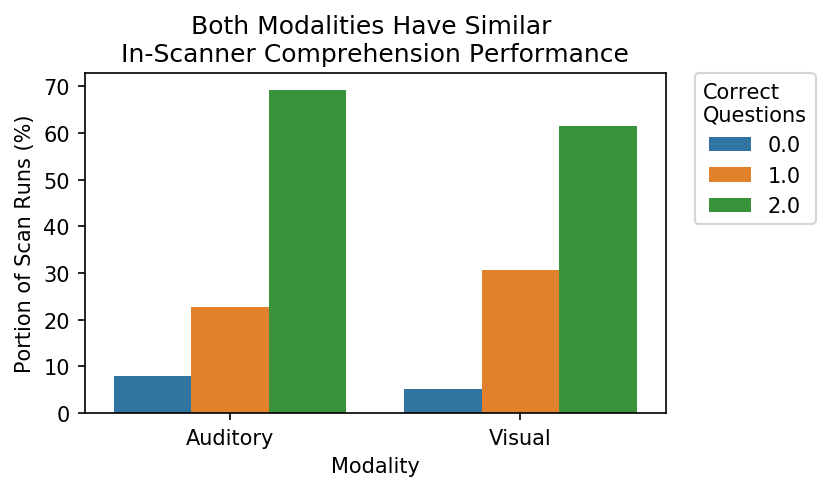
\includegraphics[width=5in]{ch2-eprime-comprehension}
    \caption[In-scanner comprehension performance did not differ by modality.]{}
	\label{fig:ch2-eprime-comprehension}
\end{figure}

\subsection{Activation results}

A range of language-related areas were activated for both reading and listening comprehension (Fig. \ref{fig:ch2-passages-activation-attn}). Compared to the corresponding sensory baselines, activation spanned the inferior frontal gyrus, angular gyrus, premotor cortex, middle temporal gyrus and the superior frontal gyrus. Activation patterns were robustly present on both hemispheres, but had greater intensity and extent on the left hemisphere. 

\begin{figure}[tp]
	\centering
	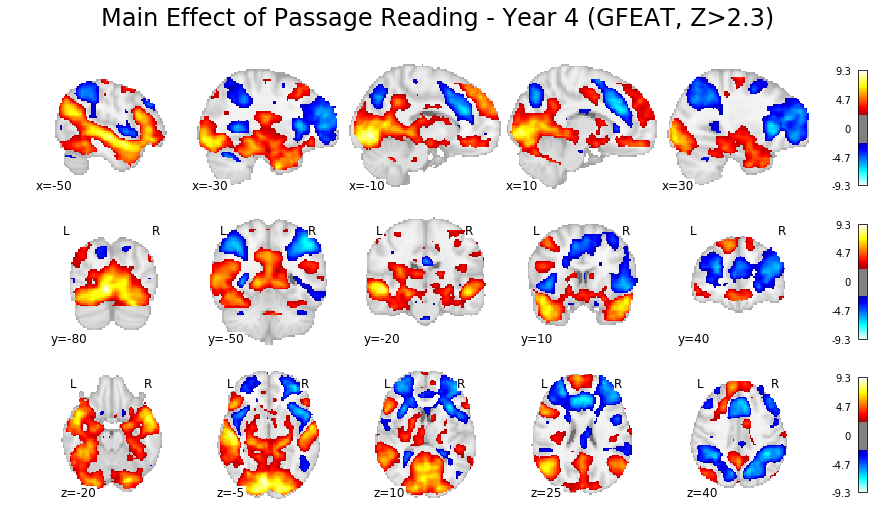
\includegraphics[width=5in]{ch2-passages-activation-attn}
    \caption[There is significant overlap between the areas used in listening and reading.]{A widespread set of brain areas are utilized during listening and reading, including auditory, default mode and attention areas.}
	\label{fig:ch2-passages-activation-attn}
\end{figure}

Differences related to modality fell into three categories: sensory processing areas, including the insula, superior temporal gyrus, and secondary visual processing areas; and hetero-modal association areas, most notably the inferior frontal gyrus and angular gyrus; and somato-motor regions, including the premotor cortex and lateral geniculate nucleus of the thalamus (Figure 2). Areas showing greater activation in listening were focused on primary auditory cortex and the dorsal attention network. 

\begin{figure}[!b]
	\centering
	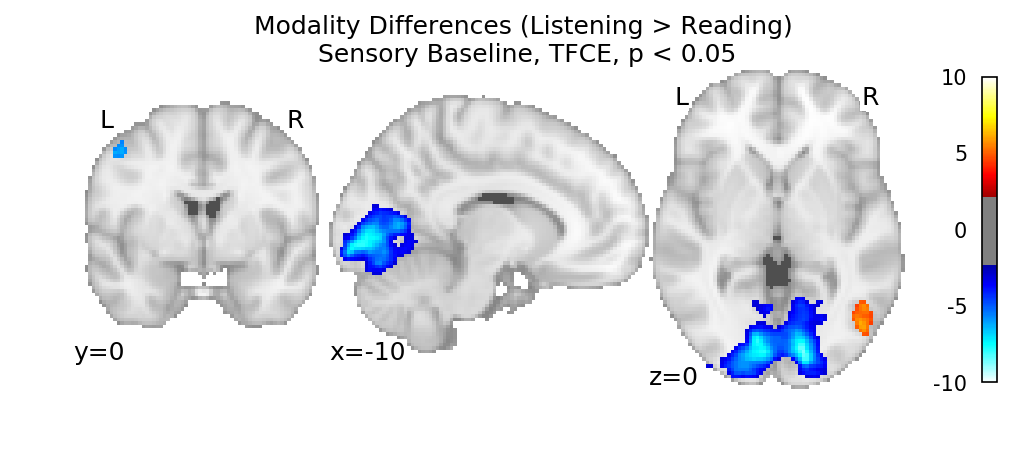
\includegraphics[width=5in]{ch2-modality-differences-attn}
    \caption[Modality differences center on primary sensory and integration areas.]{Modality differences center on primary sensory and integration areas.}
	\label{fig:ch2-modality-differences-attn}
\end{figure}



\subsection{Global graph theory metrics}

Relative to rest, both listening and reading reduced the global modularity and increased the participation coefficient. Compared to the baseline attention task, there were  trends towards an increased participation coefficient, but they were not significant. 

\begin{figure}[b]
	\centering
	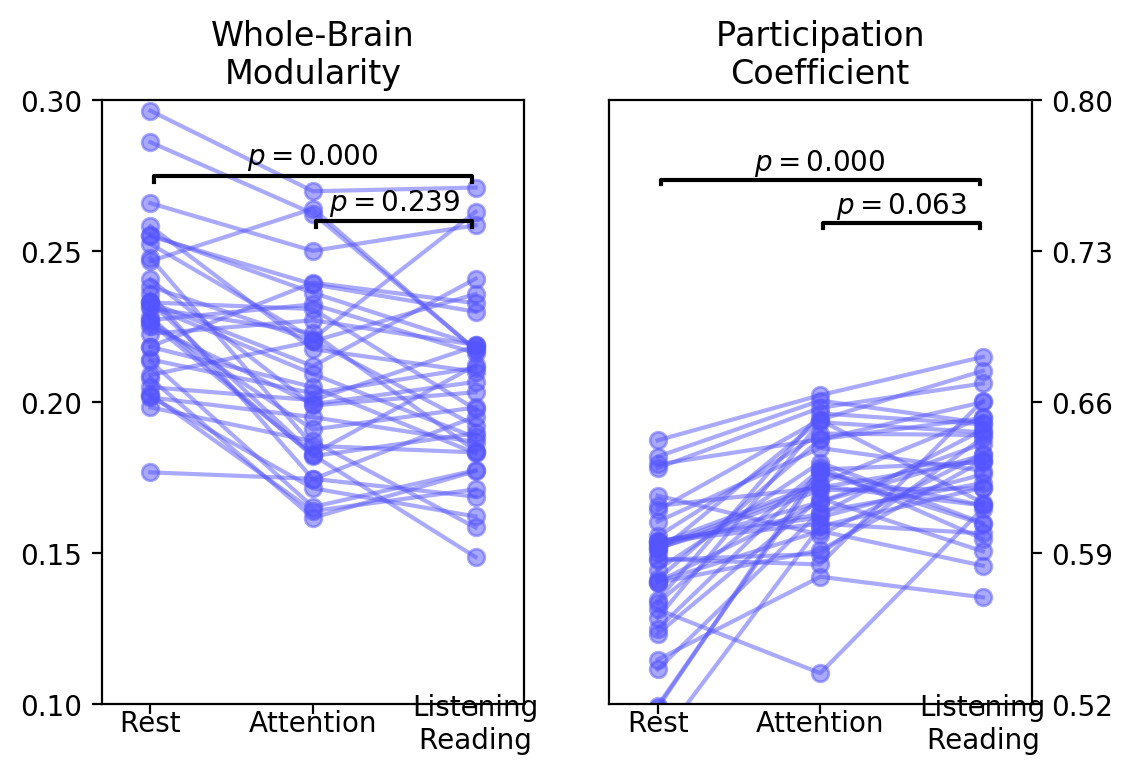
\includegraphics[]{ch2-comprehension-graph-theory}
    \caption[Language induces more integrated global network architecture.]{}
	\label{fig:ch2-modality-differences-attn}
\end{figure}

Comparing listening to reading showed that reading induced a more integrated network architecture than listening. 

\subsection{Connectivity results}


\section{Discussion}



These modality-specific influences on behavior and brain activity may arise from a few different sources: subject, linguistic and innate differences. 

\begin{itemize}
	\item \textbf{Subject-Dependent Differences:} As disussed above, reading is a learned skill with may component processes. It requires thousands of hours of experience to master and entails a reorganization of cortical resources. Environmental and biological factors thus exert a greater influence on an individual’s reading proficiency than they might on more intrinsic processes such as speech comprehension. This is particularly dramatic in individuals with dyslexia, who have persistent difficulty with reading. Children with dyslexia exhibit less activation in reading-related areas compared to typically developing children \cite{Pugh2000}, but greater activation in right hemisphere homologues, suggesting that lateralization and activation of the reading circuit are associated with better reading. Development period also has an effect, with children exhibiting less activation in frontal areas but more in posterior areas, possibly reflecting a shift in “resource load” from uni-modal to supramodal areas \cite{Berl2010}. This shift may not be necessary in listening, or occur much earlier. Thus, with increasing expertise and development, there may be a “shift” from relying on fusiform processing areas. towards using multi-modal areas more like speech \cite{Monzalvo}. 

	\item \textbf{Language-Dependent Differences:} People speak differently than they write. Reading often relies on more complicated syntax, and even for skilled readers, longer words and sentences can strain executive systems more than they might if being spoken to. Although these properties are often controlled for in scientific studies, they represent a major difference between “natural” reading and listening. Because of these differences, reading may place a greater load on executive function skills. Executive functions such as working memory and planning and organizing may be particularly important for reading \cite{Cain}.  
	
	\item \textbf{Modality-bound differences:} Speech contains overt clues about the speaker, such as tone and prosody, and these can convey additional non-linguistic meaning for the listener. Reading, on the other hand, might be considered a more purely linguistic act, especially with computer-printed text. Reading may thus allow more room for self-generated situation models and more independent direction of thought. Furthermore, modality-specific aspects of the stimulus may influence the overall comprehension process; reading requires a level of spatial awareness -where one is at on a page, what happened in preceding paragraphs – and allows for the re-treading of information. Listening, meanwhile, requires the extraction of input from competing noises and sometimes the tracking of changing volume. 
\end{itemize}

In this study, we sought to ascertain what differences existed between reading and listening comprehension of passages. We employ closely matched texts, large sample size, longitudinal sampling, and behavioral covariates. Comprehending extended text requires more than just sensory and linguistic processes. It also requires executive processes such as attention, working memory and inference. Therefore, we investigated whole-brain patterns of connectivity between different areas. 

This study pushes further than previous studies have by investigating differences between reading and listening in terms of their activation of individual areas or the distribution of activity across the brain. Since comprehension is a "whole-brain" activity, we here look at the reorganization of resting-state networks - to see how attention, executive and sensory systems are interacting during reading.

\chapter{Integration of resting-state networks during reading}

\section{Motivation}

% Reorganization may also index reading skill
In Study 1, we began building an argument that the brain compartmentalizes its cognitive functions because this improves cognitive efficiency, both for specific tasks and for integrating across the whole-brain network. We found this to be true in the case of reading fluency: global modularity is positively related to reading skill, even when controlling for verbal intelligence and motion. However, the brain network is not static but rather  changes in response to the demands made upon it. Therefore, evaluating the brain \textit{while} it is reading is critical for understanding how its organization supports fluency. 

% Task-evoked network architecture
While resting-state functional connectivity is thought to provide insights into a relatively stable intrinsic architecture, \textit{task-evoked} functional connectivity measures network organization in response to an environmental demand. The degree of reconfiguration is physiologically limited: the BOLD signal change during a task is only about 1 percent \citep{Fox2007}, and there are underlying structural constraints such as white matter connectivity \citep{Sui2014}. Nevertheless, there is a large degree of flexibility to reconfigure the functional network based on the demands of the task. One study, for example, compared a finger-tapping to working memory task. Using measures of modularity and participation coefficient, they found that within-network communication was critical for the motor task, whereas between-network communication was important for working memory \citep{Cohen2016}. This supports a hypothesis that tasks can operate on multiple levels: high connectivity within-module for sensorimotor tasks, and distributed for ones that require higher-order skills. The ability to flexibly switch between high- and low-modularity states may thus be an important trait.

% Effects on network organization during reading
Reading, and especially reading comprehension, spans both levels of cognitive activity. On the one hand, readers continuously receive visual stimuli and transform them into auditory and semantic representations. These representations must then be kept in memory, evaluated for relevance and updated when necessary \citep{Maguire1999}. In general, task-evoked network architecture induces a decrease in modularity \citep{Cole2014}, and this decrease is associated with active engagement and awareness of the task at hand \citep{Godwin2015}. Other studies have shown that the extent of the modularity is related to the novelty and expertise at the task \citep{Bassett2015}. This has not, however, been related to individual differences in those broader cognitive skills.

% Relationship of reading skill to modularity change
A complementary question is whether the relationship between reading skill and network modularity \textit{while reading} should remain the same. One hypothesis is that, if cross-network communication is critical to reading, better readers should exhibit a much less modular organization while reading than poor readers. However, there is evidence from univariate analyses of brain activation that would suggest the opposite: compared to poor readers, expert readers show \textit{less} activation in many reading-related areas during reading tasks \citep{Christodoulou2014}. In the context of interactive specialization, this is explained by the increased efficiency of information transfer within an established network. If the resting-state network architecture represents an efficient baseline, then expert readers may be expected to deviate from it less.

% How does activity relate to reading? 
It has been well-established that during reading, brain activity patterns span a wide range of networks and both hemispheres, especially as texts become longer and more complex \citep{Rimrodt2009, Xu2005}. However, less understood is the relationship between task-activity and changes to an area's role in the network. Although hub regions of the brain are known to be important for cognitive functioning, implicated in a wide variety of processes and localize predominantly onto association cortices, we are not aware of any studies that have directly compared their hub role to their BOLD response in a specific task. That is, does the ``activation'' of a hub node correspond to its connecting of more areas, or does it reflect a specific in the traditional sense corresponds to increased engagement with many areas, or if it reflects primarily local processing. The answer may be region- and task-dependent: visual areas may performing local processing, whereas activation of FPN areas may indicate the linking of two networks. 

% This study's objectives
Reading comprehension is thus an excellent model task for understanding how task-evoked changes to network architecture vary throughout the brain and along reading skill. First, we validate our task with a traditional univariate analysis. Next, we describe the global changes to different aspects of network architecture during each condition. Then, we pinpoint which brain areas and RSNs that drive the changes to network architecture, and investigate the relationship between these changes and individual differences in reading skill. 


\section{Methods}

\subsection{Participants}

Participants were drawn from the same cohort of subjects included in Study 1, and identical inclusion criteria for both demographic and scan motion were applied. However, additional measures related to the performance of the task were levied as described below. A total of 47 unique subjects and 88 scan sessions were included in the analysis. Their demographics are described in Table \ref{table:ch3-participants}.

\begin{table}
	\renewcommand{\tabcolsep}{0.09cm}
	\centering
	\begin{tabular}{lc}
\toprule 
Measure & Subjects \\ 
\midrule 
No. Participants				& 42 \\ 
No. Scan Runs					& 164 \\ 
Gender  						& 25 F \\ 
Age at Scan 					& 10.5 (0.3)  \\ 
WASI Full-Scale IQ  			& 111.0 (16.2) \\ 
TOWRE - Total Word Efficiency 	& 104.6 (18.5) \\ 
\bottomrule 
\end{tabular}
	\caption[Participant demographics for Study 2]{Participant demographics for Study 2. Subjects include all of those from Study 1, and three additional ones who had sufficiently high quality task-fMRI scans.}
	\label{table:ch3-participants}
\end{table}


\subsection{MRI acquisition and task design}

Participants performed up to four runs of a language comprehension task, which was crossed on two conditions: the modality of presentation (listening or reading) and the passage genre (expository or narrative). Functional MRI acquisition parameters were identical to Study 1 with the exception of scan duration, which was increased to a total of 250 dynamic volumes for each run. 

For the present analysis, only the ``reading'' scans were considered, and the effects of genre on brain activation were ignored, as they are balanced out within the majority of subjects. (6 subjects had only a single genre used for analysis.) In the following paragraphs, however, we will describe the experiment design in its entirety, as it will be relevant to subsequent analyses.

Each fMRI run had two baseline conditions: a modality-specific baseline task and a resting-state block with a fixation cross. At the conclusion of the comprehension portion of each experiment, two images were presented, and subjects were asked to decide if the image was related to the passage. (e.g., Is a picture of a cake with candles related to a story about a birthday party?) The order and duration for each block varied slightly across runs but was approximately: paragraph 1 (60 s), baseline 1 (60 s), paragraph 2 (60 s), baseline 2 (60 s), and resting-state (270 s). Total scan time was 550 s for each run. See Fig. \ref{fig:ch3-task-design} for a schematic describing the visual task.

\begin{figure}[t]
	\centering
	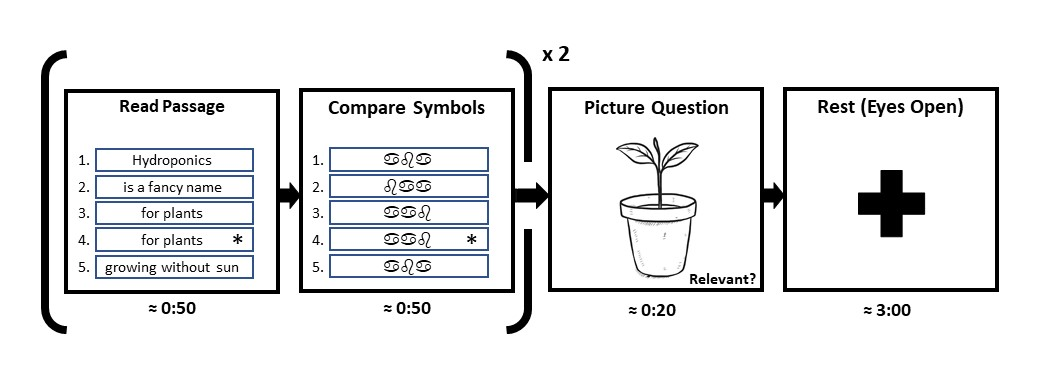
\includegraphics[width=6in]{ch3-task-design}
	\caption[Schematic of the reading comprehension task]{Schematic of the reading comprehension task. Subjects were presented two blocks of passage reading and a symbol comparison tasks, which were followed by a brief comprehension question and a resting block. Starred stimuli in the reading and symbols conditions represent ``repeat'' stimuli, and a participant is asked to click a button when they detect one. The total duration of each scan run was 550 seconds.}
	\label{fig:ch3-task-design}
\end{figure}

To create a more naturalistic reading experience than single word presentation \citep{Rayner1998}, passages were presented in syntactic phrases ranging from 1-7 words in length. The interval between each stimulus was jittered to allow for event-related analyses (range: 275 – 4000 ms), although these effects were not examined here.

The sensory baseline condition was altered according to modality. For the reading runs, three non-alphanumeric symbols were displayed horizontally (two types), and their presentation time was matched to the passage phrases. Spacing between symbols was randomly alternated to replicate the variable phrase lengths in the passage condition. For the listening runs, three tones (two frequencies) were played in sequence, with a new set of tones beginning at the same intervals as the corresponding passage presentation. 

To monitor attention, 4 to 8 percent of the stimuli within each passage or symbols block were randomly repeated on two consecutive screens.  Participants pressed a button with their right thumb when they detected a repeated phrase, symbol or tone configuration. Additionally, at the conclusion of each passage, a picture was presented on the screen, and subjects were asked to identify whether the picture had any relationship to the passage (e.g., a picture of a mushroom for a passage about fungi). 

To assess performance, we analyzed three measures: in-scanner attention, in-scanner comprehension, and post-scan recall. To assess attention for the ``repeated stimulus'' task, we used the $D`$ summary measure. It is calculated as:

$$
D^\prime = Z_{true\ positive} - Z_{false\ positive}
$$

Individual scan runs with a $D`$ value less than 2 were excluded from analysis. The in-scanner comprehension measure was the number (either 0, 1, or 2) of questions correctly answered. To assess recall after the scan, each child was asked to recite as much of the passage as they could remember, and their answers were mapped to actual phrases present in the chapter. 

In total, there were 4 passages (2 listening and 2 reading), each leveled to a third grade difficulty level and balanced on word measures such as concreteness and cohesiveness.  All subjects were trained on the task in a mock scanner prior to the actual scan. 


\subsection{Activation analyses}

Whole-brain fMRI analyses were performed using tools from the FMRIB Software Library (version 5.0.9). For each session, the following pre-processing steps were performed:  slice-time correction, motion correction to the initial fMRI volume, high-pass filtering at 0.08 Hz, boundary-based registration to the subject's structural image, and normalization to 2 mm MNI 152 standard space. To mitigate the effects of motion on our analyses, we regressed out 6 continuous motion parameters and scrubbed out outlier volumes. We defined an outlier volume as any in which the root-mean-square framewise displacement exceeded 0.7 mm. We removed scan runs where more than 20 percent of the fMRI volumes were considered outliers.

All task conditions were convolved with the double-gamma hemodynamic response function to generate design matrices for each fMRI run. Two first-level contrasts were of interest: the main effect of passage comprehension (``reading vs. rest''), and the contrast of passage comprehension vs. the sensory baseline (``reading vs. symbols''). Repeated stimuli and the picture comprehension task were modelled out.

Reading effects were estimated at the subject-level using fixed effects analysis. These were carried over into group-level analyses using non-parametric methods implemented in FSL’s \textit{randomise} tool with threshold-free cluster enhancement. For each group-level analysis, we performed 5000 permutations and report results with \textit{p} \textless 0.05. 

To understand our univariate results as a function of system-level activation, we also extracted activation values from each of the 264 connectome nodes, and summarized the activity of each intrinsic RSN.

\subsection{Network analyses}

For graph theory analyses, network estimation was performed in the \textit{Conn: Functional Connectivity Toolbox} (version 17f) \citep{WhitfieldGabrieli2012}. As in Study 1, for each scan run, the BOLD activity at each node was denoised using the anatomical CompCorr method, which regresses out background noise from white matter and cerebrospinal fluid tissue. We also regressed out 12 continuous measures of motion were also included, all outlier timepoints, and the effect of all task conditions (i.e., reading, symbols, and rest). The timeseries was then high-pass filtered at 0.01 Hz.

Whole-brain connectomes for each condition were created by estimating the functional connectivity between each node using a weighted general linear model. For connection-level analyses, these values were compared directly across subjects and conditions. For graph theory analyses, the array of all node connections was thresholded to keep the top 5 percent of connections, resulting in a much sparser representation. This threshold was also tested at ranges from 2 percent to 10 percent. These arrays were then characterized using the previously described graph theory measures: modularity, participation coefficient, and path length.

To investigate the rewiring of the network at the RSN-level, we compared the number of connections across each RSN relationship at each condition. For each pair of networks, we computed a paired $t$-test between the total number of connections between the networks to determine whether there were more in one or the other condition. This resulted in a 13 by 13 RSN-level connectivity array. Connectivity changes were performed at eaech of the 9 thresholds, and relationships that showed significant changes ($p < 0.05$, uncorrected) in at least 7 of the 9 thresholds were included in the rewiring diagram.


\section{Results}

\subsection{Behavioral results}

47 subjects (88 scan runs) met the attention and motion criteria for inclusion in the analysis. (5 subjects and 15 scan runs were excluded.) The distribution of performance and motion criteria are illustrated in Figure \ref{fig:ch3-task-performance}. 

\begin{figure}[t]
	\centering
	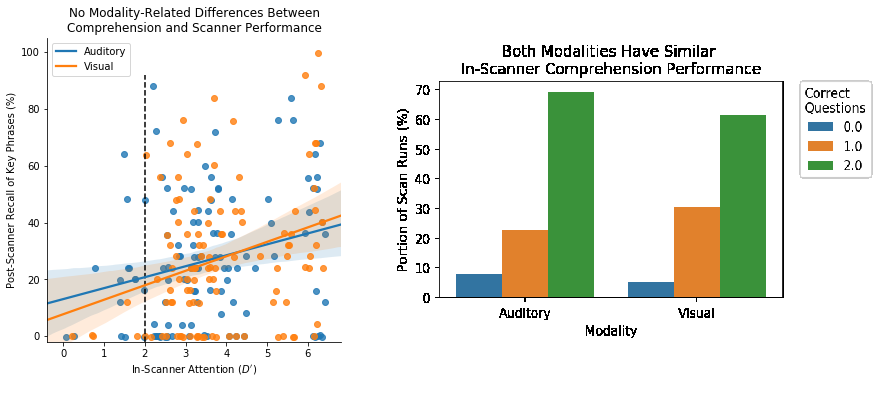
\includegraphics[height=3in]{ch3-task-performance}
    \caption[Description of scan motion quality and task performance]{Scatterplot summarizing the relationship between scan motion quality and task performance. The $D^\prime$ score measures performance based on both active (correctly identifies repeats) and passive (few false alarm clicks) metrics. The frame-wise displacement measure also accounts for outlier volumes which are regressed out during analysis.}
	\label{fig:ch3-task-performance}
\end{figure}

\subsection{Activation results}

Figure \ref{fig:ch3-reading-brain-activations} demonstrates the range of language-related areas were activated during reading comprehension. Compared to the symbols baseline, reading-related activation spanned the inferior frontal gyrus, angular gyrus, premotor cortex, middle temporal gyrus and the superior frontal gyrus. Activation patterns were robustly present on both hemispheres but extended further and with greater intensity on the left hemisphere. There were also a number of areas that were more active in the sensory and resting state, particularly in the dorsal attention network and anterior dorsolateral prefrontal cortex.

\begin{figure}[t]
	\centering
	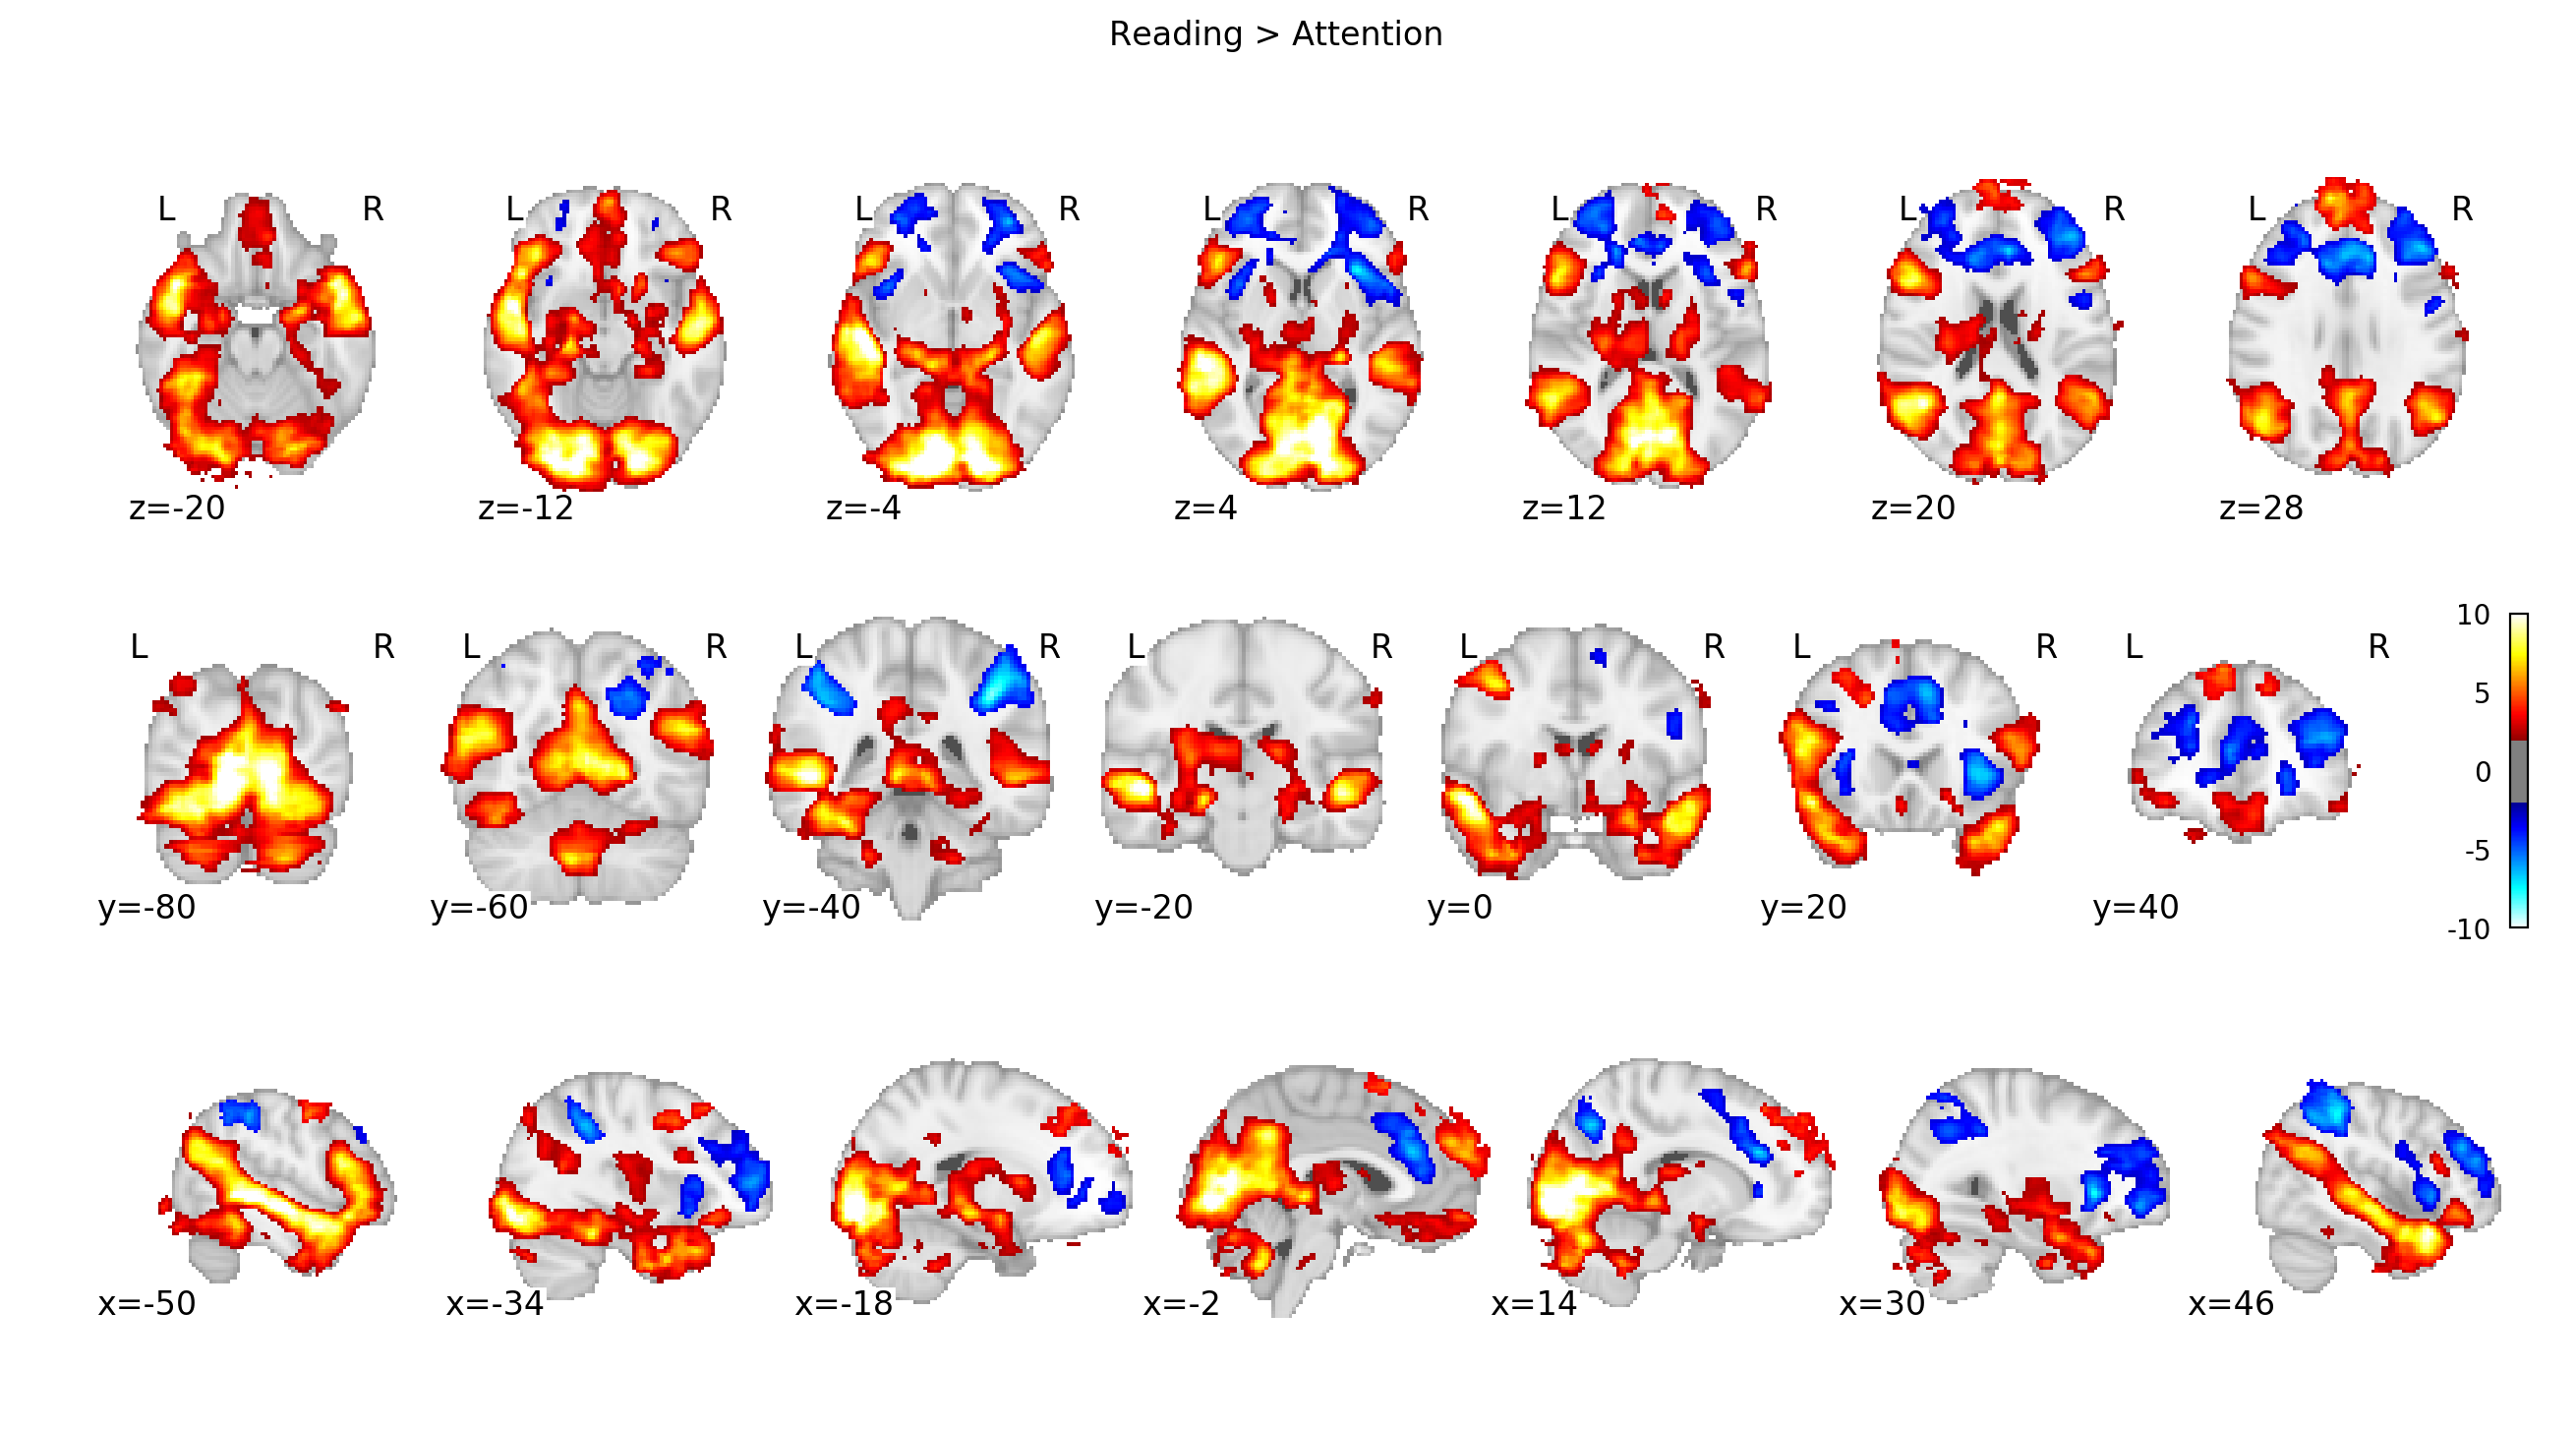
\includegraphics[width=6in]{ch3-reading-brain-activations}
    \caption[A range of language-related areas were activated during reading comprehension]{A range of language-related areas were activated during reading compreh ension. The above figures show axial, coronal and sagittal views of the ``reading vs. symbols'' activation contrast. Reading-related activations span expected areas, including left fusiform, middle temporal and inferior frontal gyri, but also extend into right hemisphere homologues and the cerebellum. Results are thresholded at $p < 0.05$ using threshold-free cluster enhancement (5000 permutations).}
	\label{fig:ch3-reading-brain-activations}
\end{figure}

To understand RSN-level trends in activation, we also examined the results when projected onto the 264 nodes in the connectome parcellation. Compared to the resting baseline, the ventral attention, visual and default mode networks had the greatest number of ``active'' nodes. It is also notable that the ``uncertain'' nodes were highly engaged. These nodes had variable activity that made them impossible to classify consistently in the original paper \citep{Power2011}. Their engagement may reflect the important role of functionally diverse regions in the execution of reading comprehension. On the other end, the memory retrieval, salience and cingulo-opercular networks exhibited decreased activity compared to rest. See Figure \ref{fig:ch3-reading-connectome-activations} for a diagram of these activations by RSN. 

\begin{figure}[t]
	\centering
	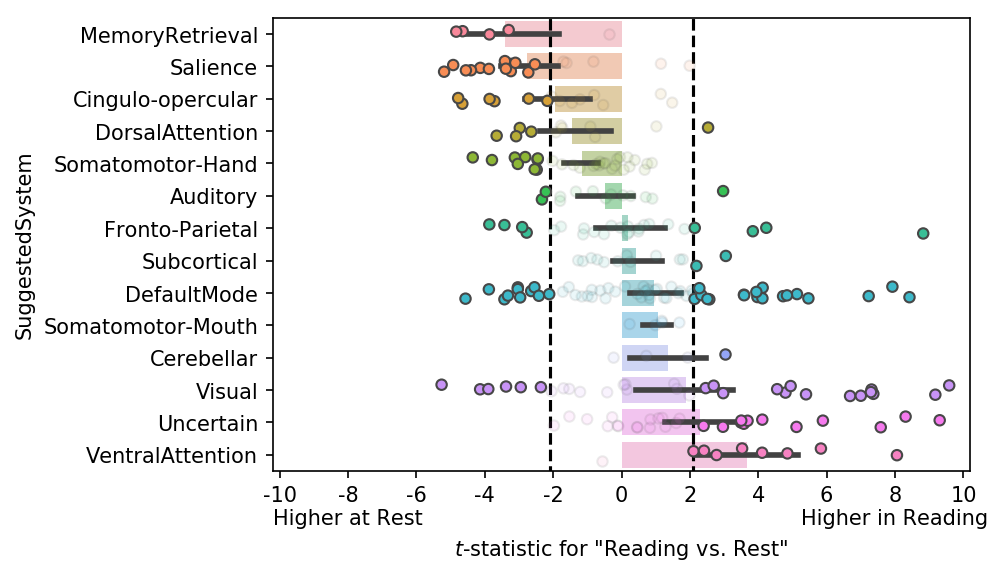
\includegraphics[height=3in]{ch3-reading-connectome-activations}
    \caption[Distribution of reading-related activity among RSN nodes]{Distribution of reading-related activity among connectome nodes, grouped by RSN. Each point represents a single node, while bars represent the aggregate mean for each RSN. Visual and ventral attention networks showed the most network-level activity in reading, although large portions of the default mode and fronto-parietal network were also robustly related. Cingulo-opercular, memory retrieval and salience networks showed decreases. Dashed lines represent $p < 0.05$, uncorrected.}
	\label{fig:ch3-reading-connectome-activations}
\end{figure}


\subsection{Network results}

Next, we examined changes to global network architecture. Figure \ref{fig:ch3-comprehension-graph-theory-all} summarizes the subject-level changes (as well as significance values) in modularity, participation coefficient, and path length. Overall, the effect was one of increased integration across RSNs during reading comprehension. Relative to rest, both reading comprehension reduced the global modularity and increased the participation coefficient. The magnitude of the effect in reading comprehension was also greater than that of the sensory condition. The path length within each RSN did not significantly change across condition, suggesting that the modular organization of the brain was not disrupted.  However, there were significant increases in the between-RSN path length corresponding to greater efficiency of transferring information between these disparate systems.

\begin{figure}[t!]
	\centering
	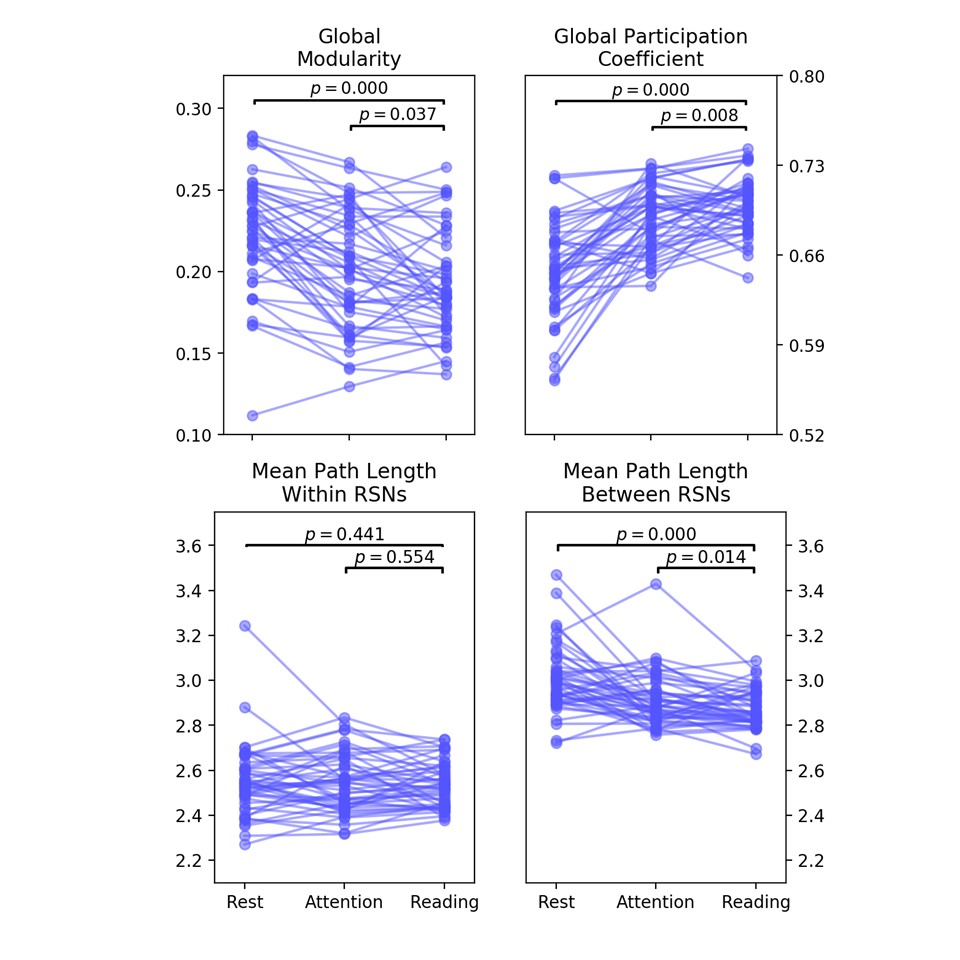
\includegraphics[width=5.3in]{ch3-comprehension-graph-theory-all}
    \caption[Reading induces a more integrated global network architecture]{Reading induces a more integrated global network architecture. Each set of connected points represents a single subject. Compared to rest and the baseline symbols task, reading comprehension increased global measures related to RSN integration. Notably, the only measure not significantly changed during task was the within-RSN path length.}
	\label{fig:ch3-comprehension-graph-theory-all}
\end{figure}

Network-level trends in task-evoked differences, presented in Figure \ref{fig:ch3-rsn-condition-effects}, were largely consistent with global effects. However, a few findings are worth noting: compared to rest, reading was marked by large decreases in modularity of the visual, dorsal attention and default mode networks. However, the increases to participation coefficient were global. Compared to the symbols task, network-level changes were modest, and the global differences were driven by reduced modularity in the default mode and fronto-parietal networks and increased participation of memory retrieval and default mode networks.

\begin{figure}[t!]
	\centering
	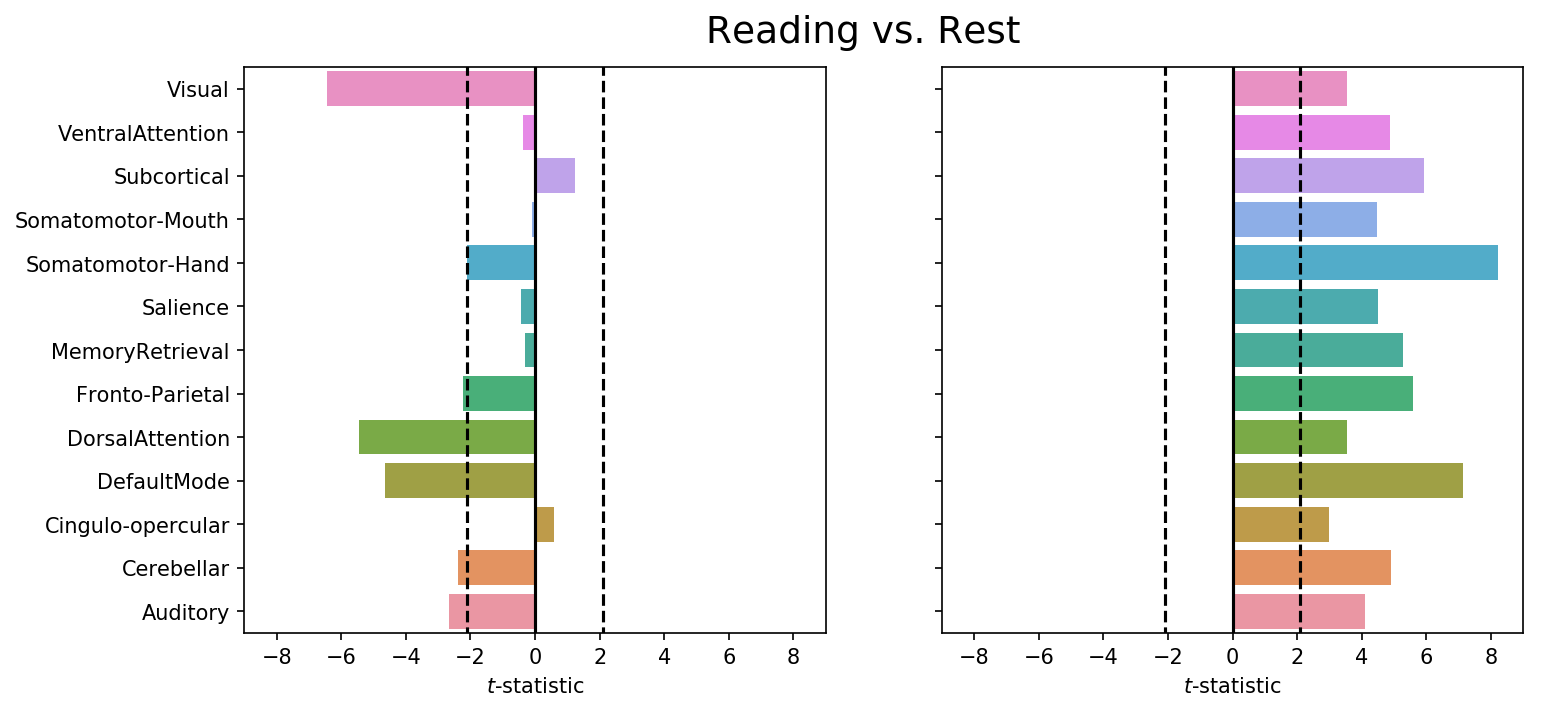
\includegraphics[width=6in]{ch3-rsn-condition-effects-rest}
	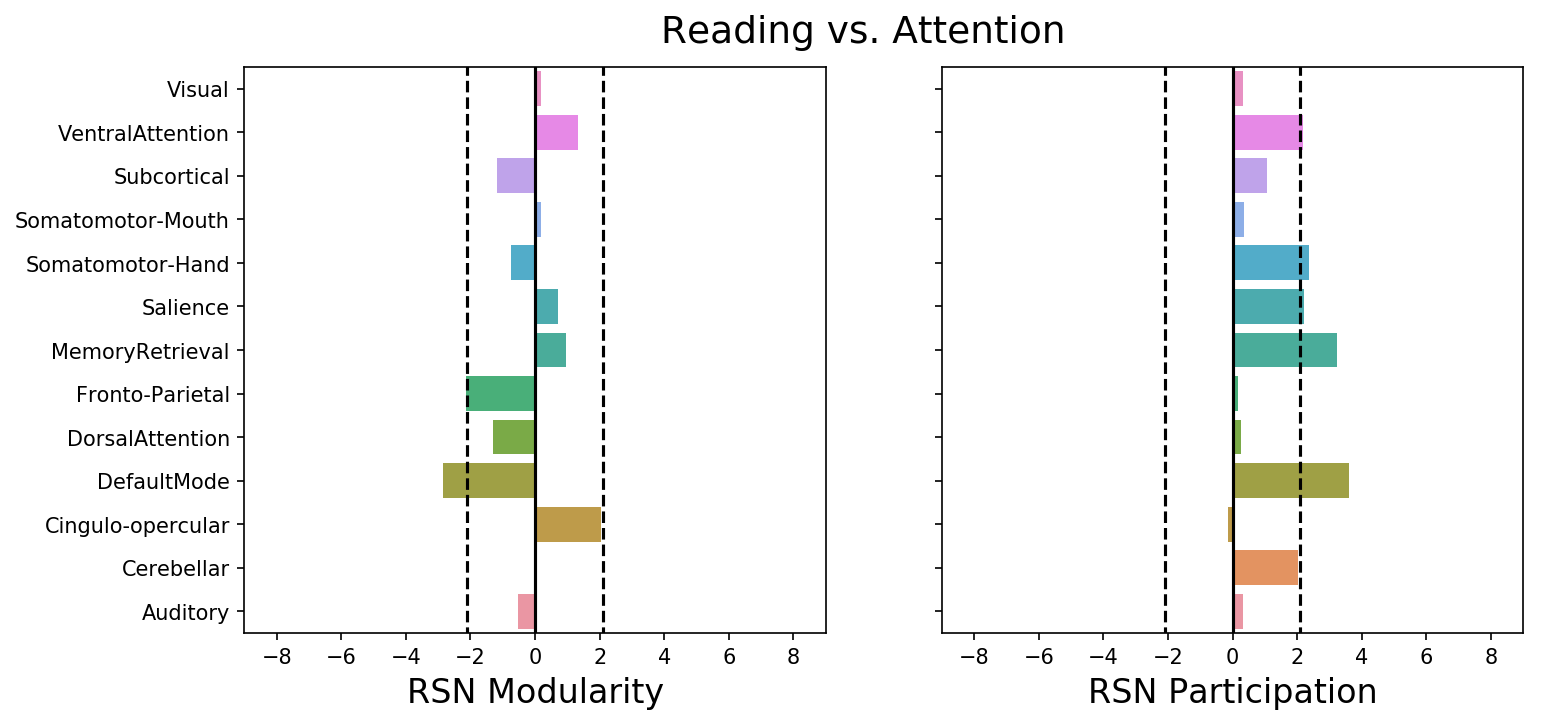
\includegraphics[width=6in]{ch3-rsn-condition-effects-attn}
    \caption[RSN-level trends in task-evoked networks]{RSN-level trends in task-evoked networks. Changes to modularity were driven by the de-clustering of the visual, dorsal attention and default mode networks. For the participation coefficient, network-level trends in task-evoked differences to graph theory measures were largely related to global trends. There were many fewer significant changes in the ``reading vs. symbols'' contrast. Dashed lines represent uncorrected significance thresholds of $p < 0.05$.}
	\label{fig:ch3-rsn-condition-effects}
\end{figure}

Specific relationships between RSNs are made apparent when comparing when examining the ``rewiring'' diagram comparing rest and reading (Figure \ref{fig:ch3-comprehension-reorganization}). During rest, there are many more within-module connections in the sensory systems, dorsal attention and default mode networks. When reading, however, between-network connections increase across many between-network relationships and none within-network relationships. There is a modest breakdown of the modularity during reading, in which there is a global increase in integration across RSNs.

\begin{figure}[t!]
	\centering
	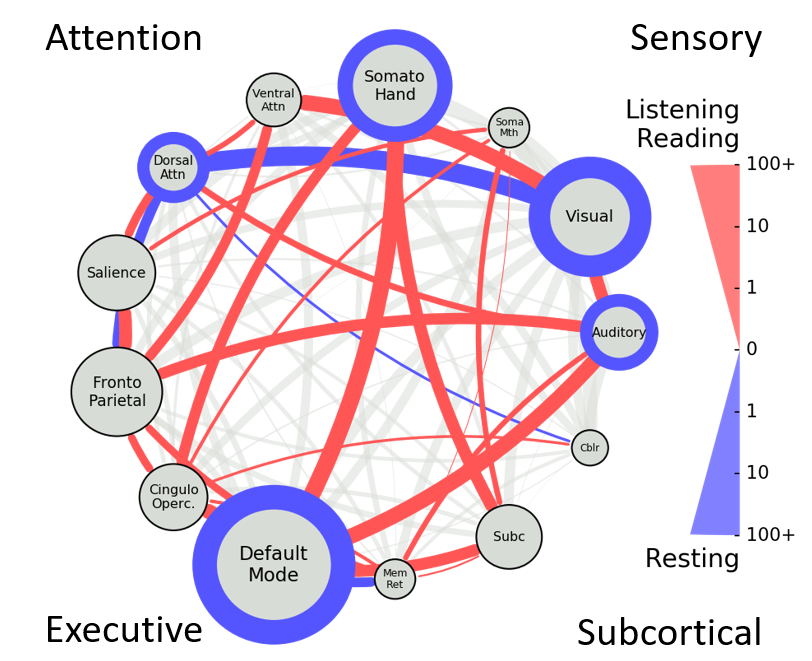
\includegraphics[height=4in]{ch3-comprehension-reorganization}
    \caption[Rewiring of RSNs during reading]{Rewiring diagram showing the changes in connectivity between networks during reading. During rest, there are many more within-module connections in the sensory systems, dorsal attention and default mode networks. During reading, however, between-network connections increase across many between-network relationships and none within-network relationships. That is, the brain becomes more integrated.}
	\label{fig:ch3-comprehension-reorganization}
\end{figure}

Decreases in modularity are coupled by increases in the participation of specific nodes. To address whether the areas that are activated during reading (in the traditional univariate sense) are also the areas driving integration, we correlated the two variables at the node level. Interestingly, we found that nodes that were more activated in reading tended to be those with lower participation coefficients ($r = -0.434$, $p < 0.001$). Nodes with high participation coefficients tended to be deactivated relative to rest, although a few of these hub-like areas were also activated. (This effect can be seen in Figure \ref{fig:ch3-node-participation-to-activation}). One noteworthy hub area was the left posterior middle temporal gyrus (MNI coordinates: $x=-56$, $y=-50$, $z=10$). It was the most hub-like area at rest ($PC > 0.7$) that was also activated during the task ($t$-stat = 8.1). 

% Color the nodes by "activated vs inactivated"
\begin{figure}[t]
	\centering
	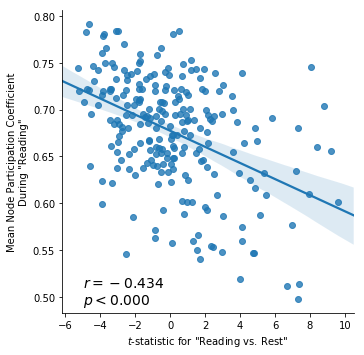
\includegraphics[width=4in]{ch3-node-participation-to-activation}
    \caption[Univariate activity is anti-correlated with participation coefficients]{Univariate activity is anti-correlated with participation coefficients. Nodes with high participation coefficients tended to be deactivated relative to rest, although a few of these hub-like areas were also activated.}
	\label{fig:ch3-node-participation-to-activation}
\end{figure}

Finally, we sought to replicate our previous finding relating resting-state modularity with reading, and to determine whether this relationship would change in the task-evoked network. For the reading and rest task conditions, we regressed the global modularity against the TOWRE Total Word Efficiency standard score. We replicated the results of Study 1 using the shorter rest condition from our task ($r_{rest} = 0.432$, $p < 0.01$), and we also found that the relationship held in the reading condition ($r_{read} = 0.494$, $p < 0.01$) (Figure \ref{fig:ch3-modularity-reading-by-condition}). There was no relationship between reading skill and the \textit{change} in modularity between reading and rest, however.  

\begin{figure}[t]
	\centering
	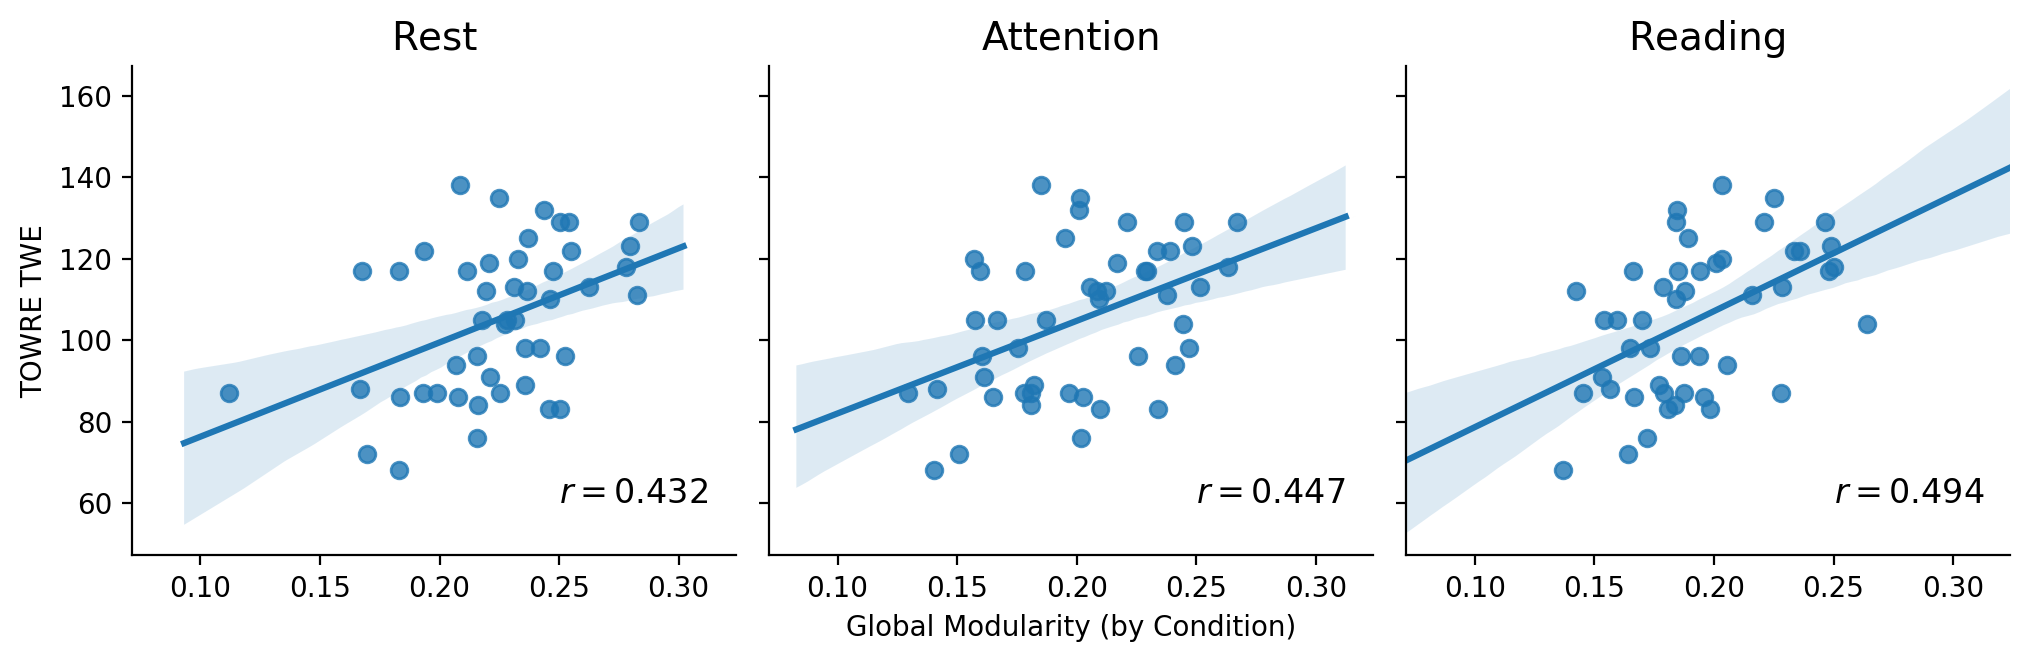
\includegraphics[width=6in]{ch3-modularity-reading-by-condition}
    \caption[Higher modularity in reading is also related to reading skill]{Higher modularity in reading is also related to reading skill. Although the global modularity significantly decreased for each subject, there was still a positive relationship between global modularity and reading skill.}
	\label{fig:ch3-modularity-reading-by-condition}
\end{figure}


\section{Discussion}

% Restatement of purpose and results
The primary purpose of the current study was to determine the ways in which task-evoked network architecture during reading differs from its baseline architecture, and whether changes in modularity are good predictors of better reading skill. As expected, we found that reading activated areas throughout the brain, especially in the visual, ventral attention and default mode networks. Reading also increased measures of integration throughout the brain compared to rest and a simple visual task. This integration was primarily driven by the de-clustering of sensory, dorsal attention and default RSNs, and global increases to the participation coefficients. Interestingly, we also found that hub areas -- those with the highest participation coefficients -- tended to be deactivated. Finally, we found that the positive direction of the relationship between modularity and reading skill was unchanged at rest and in task.

% Emphasize system-vs-laterality approach
One feature of the present connectomics approach is the disregard for laterality effects. There has traditionally been a major focus on laterality in reading and language \citep{Martin2015}. However, a systems-based approach aggregates across the RSN instead, providing a more comprehensive summary of the network's performance, but also making it less sensitive to task effects in processes that are strongly lateralized. However, there is much to be gained by prioritizing systems of the brain over sides. First, these right hemisphere regions are homologues of important left hemisphere language areas, and complement major processing areas such as the temporoparietal junction and angular gyrus \citep{Price2012, Jung-Beeman2005}. Secondly, the domain-general functions subserved by attention, executive and default networks are thought to be more global and less lateralized, so the broader scope is more appropriate when treating reading holistically (with less focus on decoding or semantics, for example) \citep{Yeo2011}.  

% Distribution of activity among different RSNs
One insight gained in this study is that much of the ``reading network'' falls predominantly in visual, default and ventral attention networks. The heavy engagement of ``unclassifiable'' border nodes is also indicative of the integrative nature of reading. While the visual and default mode networks are commonly discussed in reading comprehension as the seats of decoding and semantic processing, respectively, the attention networks have received less attention. The ventral attention network, which was the most comprehensively activated RSN in reading, plays a key role in integrating information from the environment, and regulating top-down attention. It has a push-pull relationship with the dorsal attention and salience networks. This can be seen in Figure \ref{fig:ch3-reading-connectome-activations}, where the VAN and DAN are activated in an oppposing manner. This relationship is important for reading: the dorsal attention network encompasses the visual word form area, which was the only activated DAN node and an area that has been the subject of much interest and debate in reading and dyslexia research \citep{McCandliss2003}. It is probable that this area is so important in reading not only because it is connected to language areas \citep{Bouhali2014}, but also because it is tightly tied to other areas that control goal-directed attention \citep{Vogel2014}. Vogel and colleagues found that reading ability in typical children and adults (including decoding and passage comprehension ability) predicted increased correlations between the visual word form area and the DAN \citep{Vogel2012a}. The nesting of this orthographic-processing area within the attention systems is further evidence of how fundamental global systems of attention are to the reading process.

% Changes to global modularity, but no changes to reading correlation
In terms of global network effects, we found that tasks reduced global measures of modularity and increased measures of between-RSN communication, including participation coefficient and path length. Relative to rest, this was most apparent in the visual RSN, which was characterized by a massive decrease in modularity compared to rest. These findings support a model in which the modular architecture of the brain is highly maintained between tasks, with global and some regional changes. It is not yet possible to say whether modularity within these specific RSNs correlates most highly with reading because of their functional roles in reading processes or whether they simply capture global trends better than other networks (because they are larger, for example). There is some reason to suspect specificity, however. In studies of remediation-induced changes to connectivity, increased connectivity within the visual network \citep{Koyama2013} and cingulo-opercular network \citep{HorowitzKraus2015} have predicted reading improvement in dyslexic children.

% Participation coefficient
Previous research have also noted that brain regions that have been found to be abnormal in dyslexia localize on high-hub regions \citep{Bailey2018}. It is perhaps surprising then to see primarily global effects of condition on the participation coefficient. However, this is consistent with the definition of the participation coefficient: the nodes that are increasing in participation coefficients are predominantly on the ``periphery'' of each RSN, and they are present in roughly equal proportions across all RSNs. Overall, however, we found that nodes with high participation coefficients tended not to be activated during reading, with a few exceptions such as the left posterior middle temporal gyrus. One explanation is that, in most cases, the nodes responsible for integrating information throughout the brain are not ``taxed'' in the same way that nodes performing specific computational processes are. The fronto-parietal network, for example, showed no RSN-level changes in activity, although it is known to play an important role in task-switching and coordinating neural systems \citep{Cole2013}. It is also possible that the frequency with which these hub areas are engaged varies, such that they do not activate in response to the stimuli but at other times. This anti-correlation between task activity and participation coefficient highlights the complementary nature of network analysis with activation analyses. 

% Overall significance 
Overall, the results suggest that the maintenance of an efficient network organization, i.e. one in which brain areas form clusters connected by hub regions, is important for skilled reading, even as between-network connectivity increases. To our knowledge, this is the first time the relationship between modularity and hubness to reading skill has been described during reading, adding to a foundation of work built on other connectivity methods. It also provides a replication of the resting-state findings described in Study 1. However, one limitation of the present approach is that effects were measured at a global level using the a pre-defined RSN parcellation. While this allows for reproducibility and an interpretable RSN ``rewiring'' framework, it cannot capture or describe the presence of new communities \citep{Power2011}. Comparing the modularity or individual connections between conditions assumes a reference framework, but to what extent is \textit{flexibility} in network connectivity important? Other analytical methods, such as investigating the number of shared connection between two connectomes may provide a more detailed insight into variability in task-evoked connectomes \citep{Petersen2015}. In the next chapter, we will address this question of how individual networks reorganize across a wider variety of tasks.

\chapter{Network flexibility and consistency across tasks}

\section{Motivation}

Is cognitive flexibility mirrored by functional network flexibility? That's the question we are now led to ask. In Study 1, we established that the degree of global modularity -- a key component of an efficient small-world architecture -- at rest is positively associated with reading skill. The exception to this was in the cingulo-operculuar and auditory networks, which had a negative correlation; that is, lower segregation of these areas was associated with better reading. In Study 2, we found that reading comprehension induced a more integrated network architecture as information was shared across RSNs. However, the relationship between reading skill and modularity persisted, even as connectomes were estimated during separate conditions. 

Thus, it appears that flexibility in functional networks -- at least those constructed using functional MRI -- across different tasks may not be related to efficiency of cognitive processing. Rather, better readers seem to have a shared and strong network ``backbone'' that is persistent throughout task reconfiguration. One way to test this in the context of reading would be to quantify the degree of reconfiguration (or conversely, similarity) between the task-evoked architecture. Given that reading is a skill that we know requires a very high degree of cross-RSN interaction, we might expect this to be true in a variety of other domains as well. In fact, we might expect that there would be a high degree of consistency between a number of different tasks: listening and reading, but also more basic attention and resting states. 

In this third study, we expand our task and analyses to encompass the auditory modality in order to address two questions. First, do better readers have greater similarity between different language comprehension conditions? Second, to what extent does flexibility in network organization predict individual differences in reading skill and cognition? Below, we motivate these two aims individually.

\subsection{The connectome in language comprehension}

The most widely-held view is that reading and listening share the same core linguistic processes and differ primarily in the sensory processes that feed into supra-model linguistic systems \citep{Mattingly1971, Price2012}. One popular model, the \textit{Simple View of Reading} states that reading comprehension is the product of listening comprehension and decoding skills \citep{Gough1986}. This view has received support from large behavioral studies \citep{Kirby2008} and neuroimaging investigations: many of the literacy-related changes are linked to visual or phonological systems, areas not directly related to semantic or comprehension processes \citep{Schlaggar2007, Dehaene2015}. These findings support a model in which inputs from auditory or visual domains are fed up into higher-order association areas that sequence, encode articulation plans, and extract semantic information \citep{Price2012}. These processes localize onto the similar areas regardless of language and writing system \citep{Rueckl2015}, and may even extend to inputs from somatosensory domains \citep{Xu2005, Sood2016}. This supra-modal language core is largely left-lateralized and centers on the inferior frontal gyrus, anterior and posterior middle temporal gyrus and the angular gyrus. Neuroanatomical models of language, for example the one shown in Figure \ref{fig:ch4-price-language-models}, illustrate that language is distributed throughout much of the brain with a high degree of overlap between listening and reading comprehension. 

\begin{figure}[t]
	\centering
	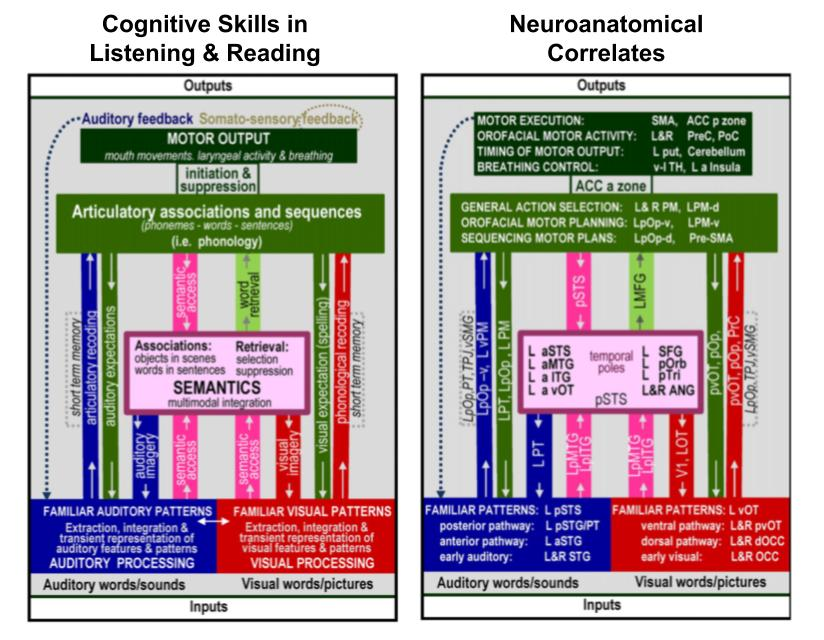
\includegraphics[width=6in]{ch4-price-language-models}
    \caption[Common core architecture for reading and listening]{There exists a common core architecture for reading and listening. The models presented here contend that reading and listening share the same core processes, with the major differences being in the sensory processing functions. Figure adapted from \citep{Price2012}.}
	\label{fig:ch4-price-language-models}
\end{figure}

Most cognitive models suggest that language comprehension requires the construction of a mental representation that includes textual information and associated background knowledge, connected by some conscious and some unconscious executive processes \citep{Kendeou2014}. During comprehension, the relationship between areas is dynamic and constantly being re-evaluated. The roles of attention and executive systems are likely to play an important role. Thus, while there may be a core set of systems for manipulating and extracting meaning from language, it is likely that differences in modality would modulate these processes. 

Despite the clear overlap between reading and listening, there is also evidence that the two skills are not directly equivalent. The pioneering researcher Alvin Liberman suggested that reading is parasitic on listening: it requires the majority of the listening machinery, as well as an awareness of the linguistic act \citep{Mattingly1971}. There is a subset of students who, despite adequate word decoding skills and vocabulary skills, struggle with reading comprehension \citep{Pimperton2010, Spencer2014}. From a neurobiological perspective, expected differences in primary visual areas (for reading) and primary auditory areas (for listening) represent the different input systems, with ventral occipito-temporal systems also activating \citep{Jobard2007}. However, differences in core language systems are also observed: additional activation in left posterior temporal and parietal areas in reading modality \citep{Constable2004}, as well increased bi-laterality especially in children \citep{Berl2011}. Altogether, there is substantial evidence that reading relies on existing speech comprehension circuitry. Therefore, a \textit{convergence} in the evoked networks may be an indicator of better reading.

\subsection{The connectome across many tasks}

As seen in Chapter 3, global and regional network architecture changes during task activation, but it preserves its overall modular structure nonetheless \citep{Cole2014}. A subsequent question is, what attributes of the network architecture enable flexibile reorganization while also preserving modularity? Strong candidates for this role are hub regions, but these should also show flexibility across a number of tasks -- not just listening and reading but other cognitive tasks as well. 

The ``flexible hub'' theory asserts that a subset of regions in the brain are responsible for coordinating other brain systems in the accomplishment of internally-directed aims \citep{Cole2007}. Hubs provide a way in which the brain might maintain its overall modular architecture while still increasing communication between regions. While there are a number of cognitive systems that may perform hub-like functions, including the salience, dorsal attention, ventral attention, and cingulo-opercular networks, several researchers have targeted the front-parietal network as a particularly important set of areas likely to perform hub-like functions \citep{Cole2013, Niendam2012}. 

The frontoparietal network is an assembly of brain regions encompassing the lateral frontal and parietal cortices along with insular, anterior/mid cingulate, and inferior temporal areas that have been broadly implicated in a variety of higher-level cognitive tasks \citep{Fedorenko2013}. One reason it has been targeted is that it encompasses the lateral prefrontal cortex, which has been seen to exert top-down control over other brain areas and which is often active in novel or difficult tasks \citep{Duncan2010}. Some have described the frontoparietal network as supporting active and adaptive online control, initiating and adjusting goal-directed mental systems \citep{Dosenbach2007}, while others have proposed a more general superordinate role in directing cognition \citep{Niendam2012}.  Global functional connectivity in the fronto-parietal network has also been shown to predict individual differences in cognitive skills and intelligence \citep{Cole2011}. Taken together, there is significant evidence for the importance of hub regions in supporting flexible cognition, and the fronto-parietal network may be particularly important. 

\subsection{Study aims}

On the one hand, we have evidence that modularity within the global network, in any condition, is predictive of reading skill. On the other hand, we know that different skills rely on different brain areas and require different systems to coordinate. Therefore, the aims of the present study were to determine to what extent flexibility across different tasks is predictive of individual differences in skilled reading.  First, we test \textit{similarity} between listening and reading network architecture corresponds to higher reading skill. Second, we examine whether \textit{dissimilarity} among resting-state networks across many conditions will correspond to higher reading skill (that is, variability in connectivity). We expect that this dissimilarity will be most present in associative RSNs such as the fronto-parietal network. 


\section{Methods}

\subsection{Participants}

Participants were drawn from the same cohort of subjects included in Studies 1 and 2, and identical inclusion criteria for both demographic and scan motion were applied. However, additional measures related to the performance of the task were levied as described below. A total of 42 unique subjects and 142 scan sessions were included in the analysis. The demographics for these subjects are described in Table \ref{table:ch4-participants}.

\begin{table}[t]
	\renewcommand{\tabcolsep}{0.09cm}
	\centering
	\begin{tabular}{lc}
\toprule
Measure &               Value \\
\midrule
Subjects                        &              42 \\
Mean age                        &    10.51 (0.33) \\
Sex                             &      21 M, 23 F \\
WASI Full-Scale IQ, Vocabulary  &    52.91 (9.38) \\
Test of Word Reading Efficiency &  104.66 (18.07) \\
\bottomrule
\end{tabular}
	\caption[Participant demographics for Study 3]{Participant demographics for Study 3. Participants were a subset of those examined in Study 2, who had also completed a listening comprehension task with sufficiently high quality.}
	\label{table:ch4-participants}
\end{table}

\subsection{Functional MRI acquisition and processing}

The task design for this study is described in detail in Chapter 3. Briefly, subjects were presented up to four separate runs of a language comprehension task. The task included two passage blocks (``reading'' or ``listening''), two sensory baseline blocks (``symbols'' or ``tones'') and a trailing resting-state block (``rest''). The four scan runs were crossed on two conditions: the modality of presentation (auditory or visual) and the genre of the passage (narrative or expository). 

A scan session was excluded based on the following parameters: the number of high-motion volumes exceeding 20 percent, mean frame-wise displacement greater than 0.4, or poor task performance ($D^\prime < 2$). To control for the effects of genre, we matched all scans that met inclusion criteria with their opposing-modality counterpart, so that each subject had either 2 scans (same genre in listening and reading) or 4 scans (both genres in listening and reading). In total, 42 children (142 scans) met inclusion criteria.

Functional MRI acquisition and preprocessing procedures were equivalent to those described for Study 2. See the \textit{Methods} section of Chapter 3 for a detailed description of these processes and their parameters.

\subsection{Activation and network analyses}

Our analysis was broken into two parts: first, comparing the similarities and differences in network organization for listening and reading, then across all available tasks. 

For the modality comparisons, we used a fixed-effects subject-level model to estimate the shared activation for ``listening and reading'' and their differences ``listening vs. reading''. We then used FSL's \textit{randomise} utility to estimate the main effects of modality across all subjects in our sample (5000 permutations, threshold-free cluster enhancement, $p < 0.05$).  We also investigated these effects in ``connectome space'' by extracting the values at each of the 264 nodes used for connectivity analysis, then comparing the activity profile of each RSN during reading and listening.

\subsection{Network similarity estimation}

Global modularity estimates the similarity of a network to a reference partition, such that two networks with high modularity must be similar to the reference, but not necessarily to each other. This method, while useful, has the drawback of being biased towards the provided RSN parcellation: two networks could receive the same modularity score, but deviate in significant ways (i.e. both similar to partition but not to each other). 

\begin{figure}[t]
	\centering
	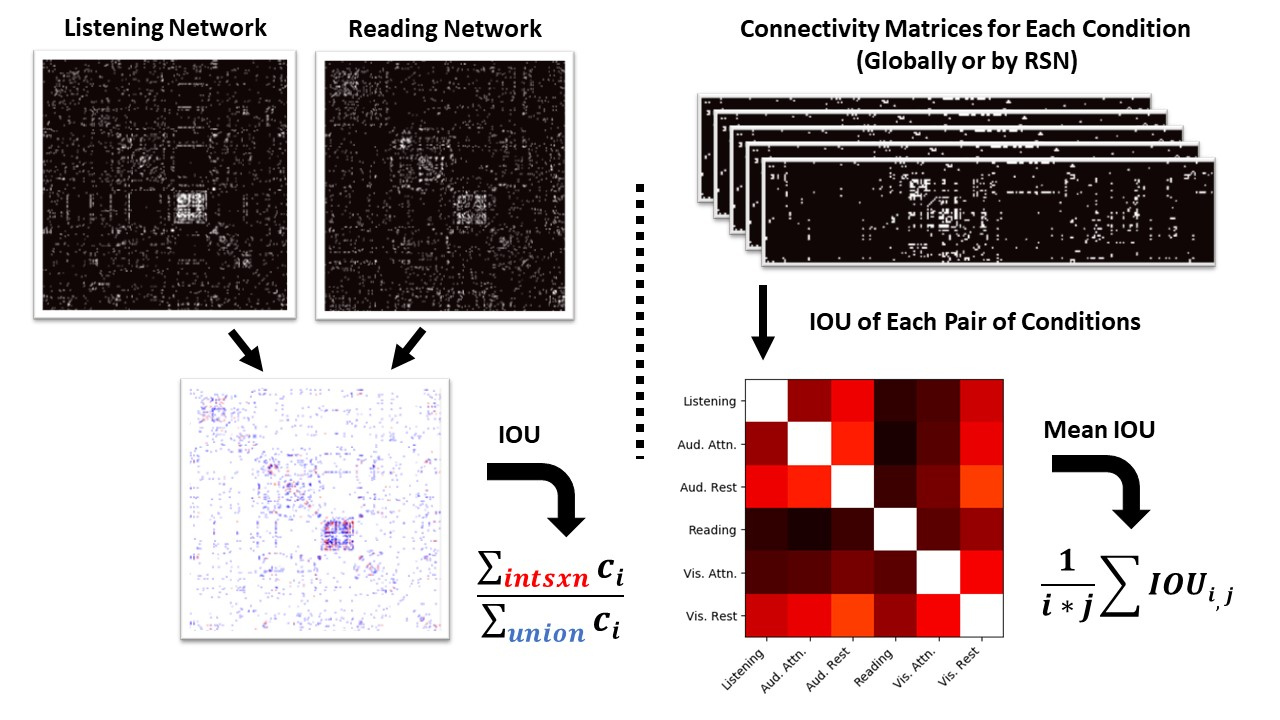
\includegraphics[width=6in]{ch4-network-similarity-methods}
    \caption[Methods for measuring similarity between whole-brain connectomes]{Schematic of methods for measuring similarity between whole-brain connectomes. The intersection of the union (IOU) can compare two connectivity arrays without reference to a pre-defined set of RSNs. On the left are methods for comparing listening to reading connectomes. On the right are methods for comparing, for each whole-brain network or RSN array, the similarity across all all task and rest conditions.}
	\label{fig:ch4-network-similarity-methods}
\end{figure}

One similarity metric that is not biased towards a reference is the \textit{intersection of the union} (IOU). To calculate the IOU of two binary matrices, one sums the total number of shared connections (intersection) and divides it by the total number of connections in either array (union), resulting in a value between 0 to 1, with 0 corresponding to no shared connections and 1 representing identical arrays. IOU provides two advantages compared to simply calculating the number of shared connections: it converts all comparisons to a common range, and it can compare arrays with different numbers of connections without being biased towards dense arrays (e.g. comparing an array with many connections to one with few connections). The IOU approach provides a complementary perspective to estimates of modularity.

We first compared the IOU of network arrays across individuals within the two linguistic conditions: listening to listening and reading to reading. We summarized the distributions of the IOU, with the expectation that there would be the most variability within the reading condition, since listening is more ``natural''. Next, we tested whether the similarity between an individual's reading and listening network arrays was related to reading skill. Finally, we analyzed RSN-level patterns of similarity and difference between reading and listening. 

Next, we broadened the scope of analysis to include comparisons between all task conditions: rest (x2), symbols, tones, listening and reading. For each subject, we calculated the IOU between each evoked network in all conditions. This resulted, for each subject, in 15 network comparison values, for each set of nodes examined. The question we were interested in was whether, within-subject, individuals who had fewer changes in network configuration were also better cognitive performers. We then sought to determine whether changes within a single RSN (e.g. the fronto-parietal network) were the key drivers of this. 


\section{Results}

\subsection{Behavioral results}

Attention and comprehension measures were not related to modality of stimulus presentation. There was a trend towards difference in median FDRMS between scan modalities (paired t-test, $t = 1.904$, $p = 0.059$), so we also replicated analyses with a stricter motion threshold (no more than 10 percent outliers in a scan run). The main results from analysis of this 35 subject (116 scan runs) cohort were broadly consistent.

\subsection{Activation results}

As expected, reading and listening shared a common core of language-related activations. These included the bilateral middle temporal and inferior frontal gyri, as well as the  anterior temporal poles. The differences related to modality fell into three categories: sensory processing areas, including the insula, superior temporal gyrus, and secondary visual processing areas; and hetero-modal association areas, most notably the inferior frontal gyrus and angular gyrus; and somato-motor regions, including the premotor cortex and lateral geniculate nucleus of the thalamus (Fig. \ref{fig:ch4-modality-comparison-attn}). Areas showing greater activation in listening localized on primary auditory cortex and the dorsal attention network.

\begin{figure}[t!]
	\centering
	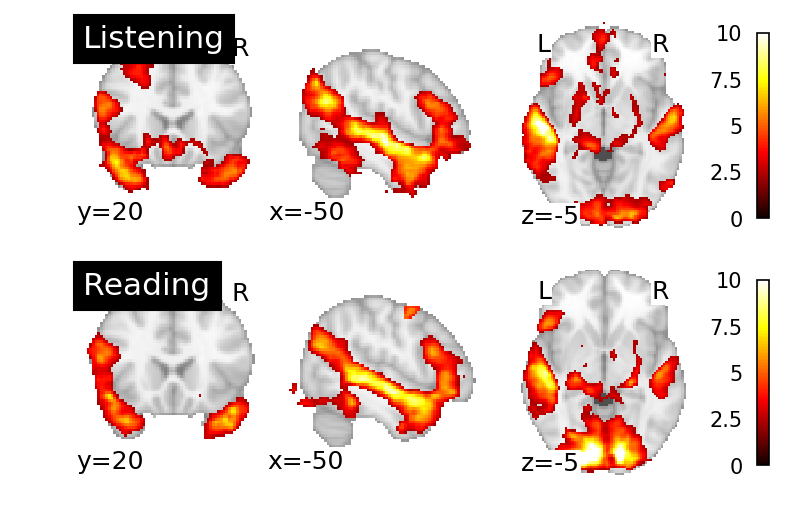
\includegraphics[height=3in]{ch4-modality-comparison-attn}
	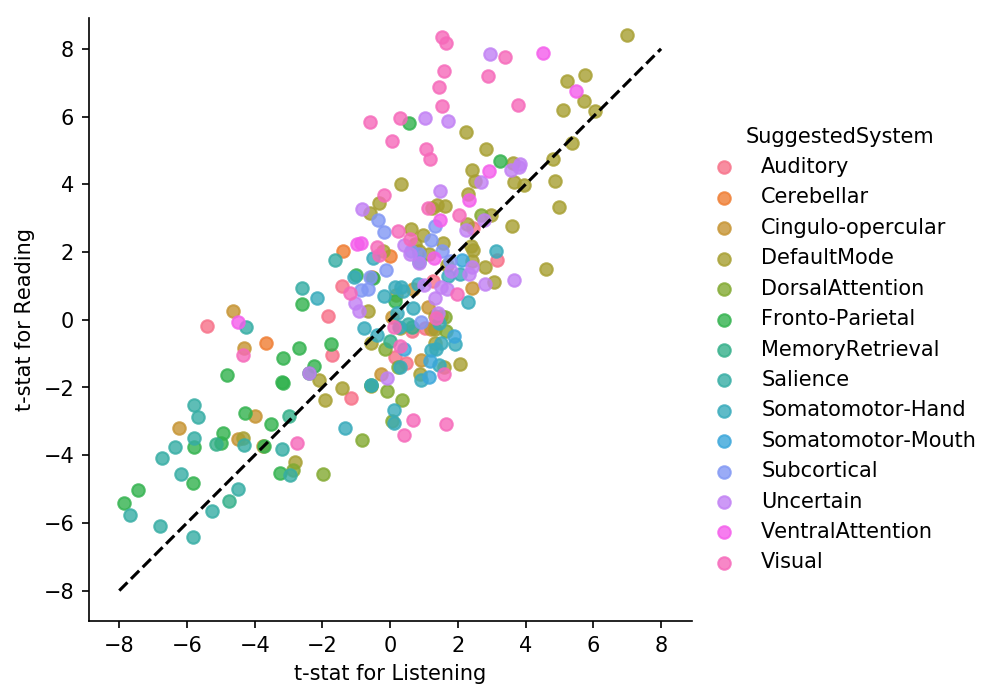
\includegraphics[height=3in]{ch4-listening-reading-connectome-activation-attn}
    \caption[Large overlap between listening and reading activation]{There was a large overlap in activation between the listening and reading comprehension tasks. Activation spanned a bilateral set of regions, especially around middle temporal, inferior frontal gyri. Activations shown for $p < 0.05$, threshold-free cluster enhancement (5000 permutations).}
	\label{fig:ch4-modality-comparison-attn}
\end{figure}

This result is more easily visualized when viewing it in terms of the 264 nodes of the connectome. There was a very high correlation coefficient between activation during reading and listening compared to the sensory baseline ($r = 0.748$, $p < 0.001$), reflecting the high degree of shared activity in the language network. Relative to rest, the variability was slightly higher ($r = 0.552$, $p < 0.001$), but still significant. 

In general, areas that are active during listening are also active during reading, but there were differences in the intensity with which they were activated: many nodes were more strongly activated in reading compared to listening. Figure \ref{fig:ch4-listening-reading-network-activation-attn} displays these in connectome space. These fell predominantly into the ventral attention, visual, and default mode networks. Only a few areas were more active in listening than reading: areas in the dorsal attention network and a few in the default mode and salience networks. 

\begin{figure}[t]
	\centering
	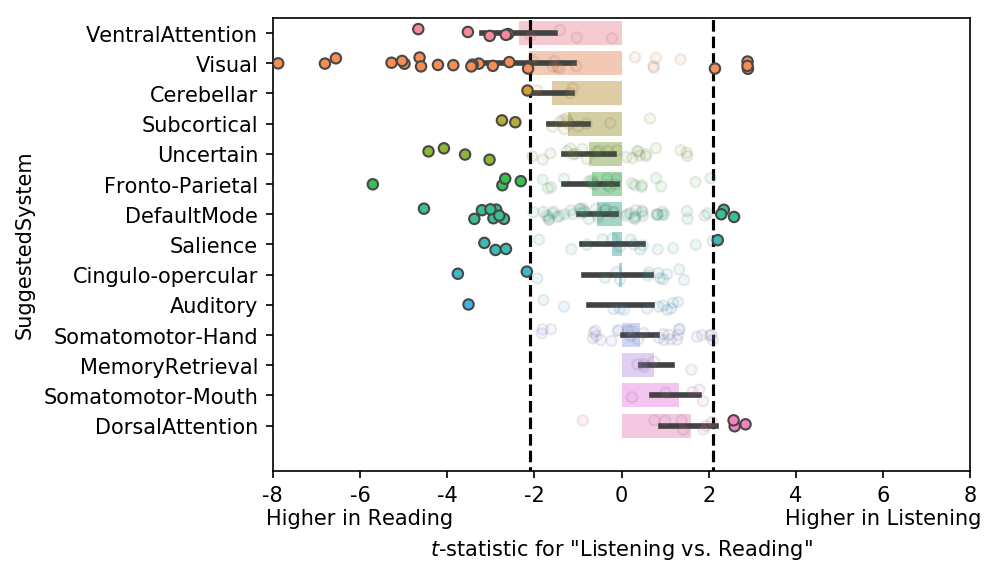
\includegraphics[height=3in]{ch4-listening-reading-network-activation-attn}
    \caption[Activation differences due to modality of presentation among RSNs]{Activation differences due to modality of presentation among RSNs, when both tasks were compared to their sensory baseline. Each point represents a single node, while bars represent the aggregate mean for each RSN. Visual and ventral attention networks showed the most network-level activity in reading, although large portions of the default mode and fronto-parietal network were also robustly related. Cingulo-opercular, memory retrieval and salience networks showed decreases. Dashed lines represent $p < 0.05$, uncorrected.}
	\label{fig:ch4-listening-reading-network-activation-attn}
\end{figure}

\subsection{Network results}

In terms of graph theory measures, we found a significant decrease in modularity ($t = 3.670$, $p < 0.001$) and a significant increase in participation coefficient ($t = -4.312$, $p < 0.001$) in reading compared to listening (top panel of Figure \ref{fig:ch4-modality-graph-theory}). Investigating the differences in path length between the two modalities provides a stronger sense of key drivers of this increased integration. The bottom panel of Figure \ref{fig:ch4-modality-graph-theory} displays the node-level connections of nodes that get closer or further during the reorganization. The large amounts of red reflect the greater global integration seen in reading; the blue patches represent a reduction in modularity within visual networks especially.

\begin{figure}[t!]
	\centering
	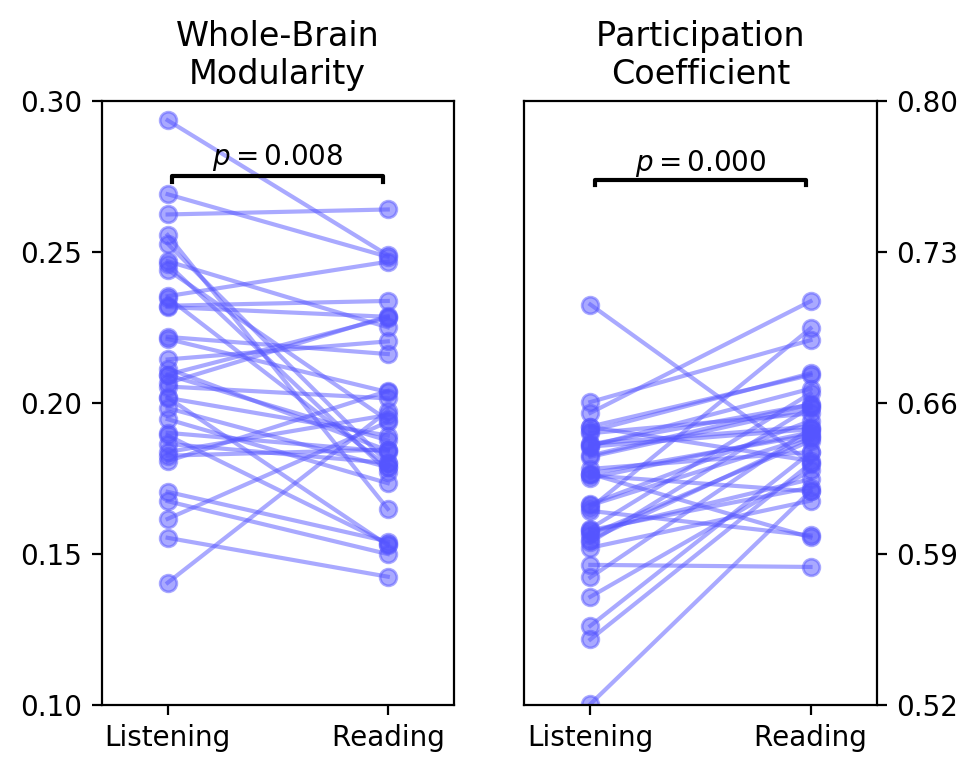
\includegraphics[height=3in]{ch4-modality-graph-theory}
	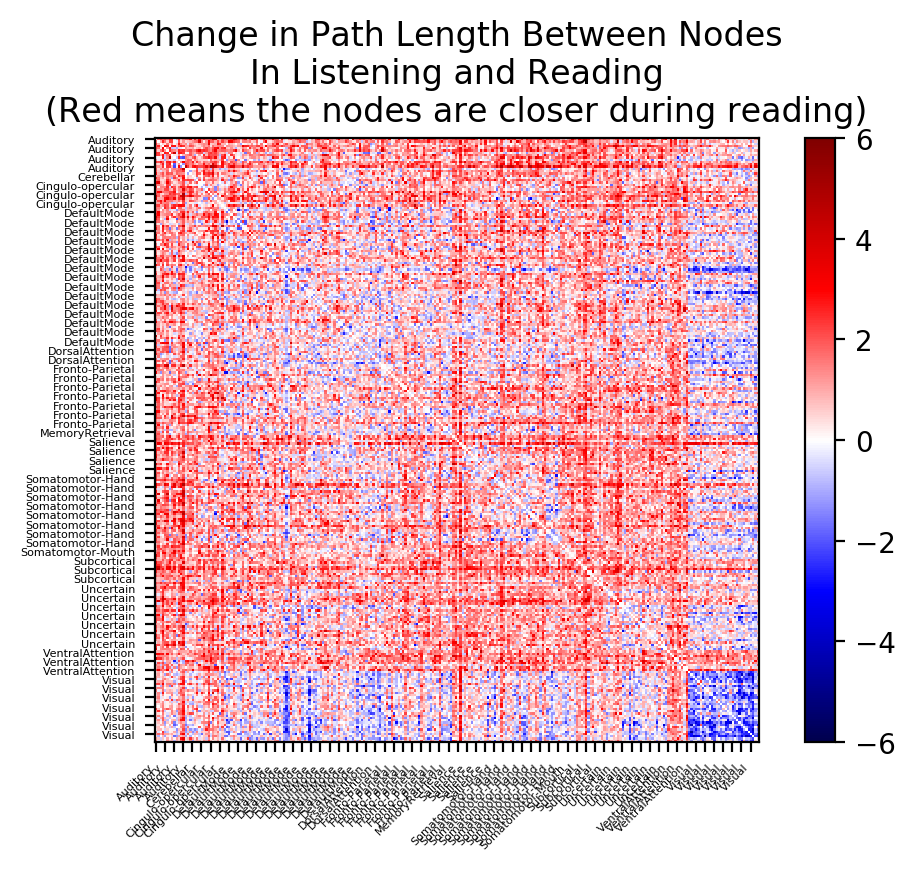
\includegraphics[height=3in]{ch4-modality-node-distance}
    \caption[Reading induces a more integrated network architecture than listening]{Reading induces a more integrated network architecture than listening. In terms of modularity and participation coefficient, there is greater integration during reading than listening. The bottom panel displays the changes to the number of steps connecting each node. The large amounts of red reflect the greater global integration seen in reading; the blue patches represent a reduction in modularity within visual networks especially.}
	\label{fig:ch4-modality-graph-theory}
\end{figure}


\subsection{Network similarity results}

We next investigated whether different individuals evoked language-architectures that were similar to each other. For each pair of participants and modality of presentation, we calculated the IOU between their whole-brain networks. We found that subject connectomes were much more similar when comparing ``listening'' connectomes than when comparing ``reading'' connectomes ($t = 53.190$, $p < 0.001$). Additionally, we found that subjects with the highest mean similarity overall were also more similar to other high-similarity subjects, suggesting that they are each approximating a common architecture during the comprehension process (see top panel of Figure \ref{fig:ch4-modality-network-similarity}).

\begin{figure}[t!]
	\centering
	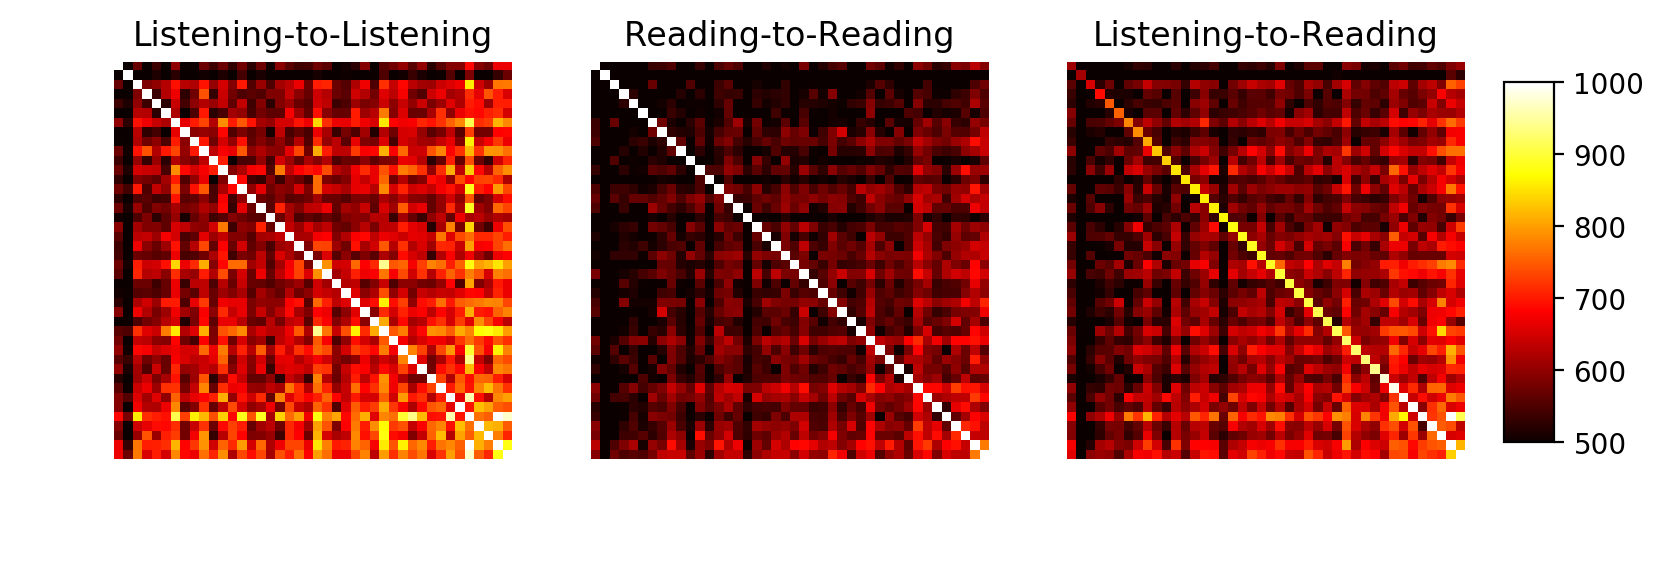
\includegraphics[width=5.5in]{ch4-modality-network-similarity}
	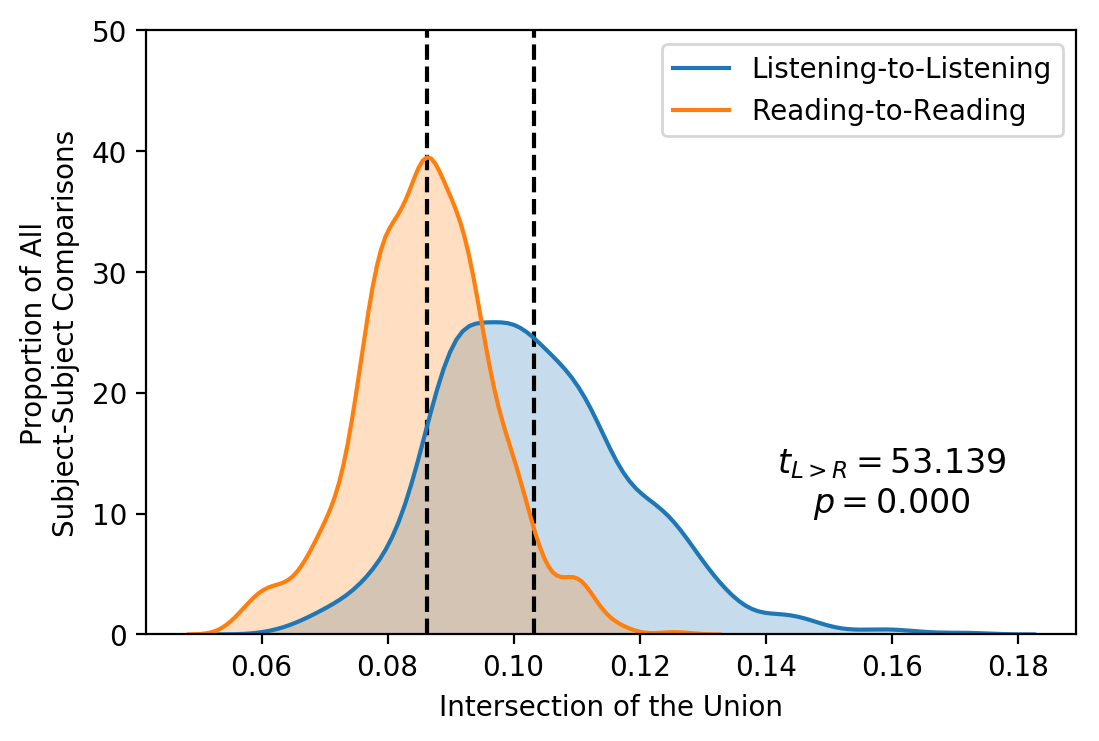
\includegraphics[width=5in]{ch4-similarity-condition-histogram}
    \caption[Network similarity across subjects in listening and reading.] {Distribution of subject similarity values in listening and reading. When comparing participant networks, there is greater similarity in listening than there is in reading (bottom). Furthermore, subjects with high mean similarity were also more similar to each other (top).}
	\label{fig:ch4-modality-network-similarity}
\end{figure}

As readers become more experienced, the expectation is that the task-evoked network architecture for reading would become more similar to that of the ``natural'' listening comprehension system. To test this, we compared each subject's listening network with their reading network then correlated this measure with TOWRE scores (Fig. \ref{fig:ch4-modality-similarity-to-reading}). Better readers did have a higher degree of similarity between the listening and reading networks ($r = 0.408$, $p = 0.007$). Furthermore, we found that reading and listening networks within a subject than between any two subjects ($t = 26.123$, $p < 0.001$). 

\begin{figure}[t!]
	\centering
	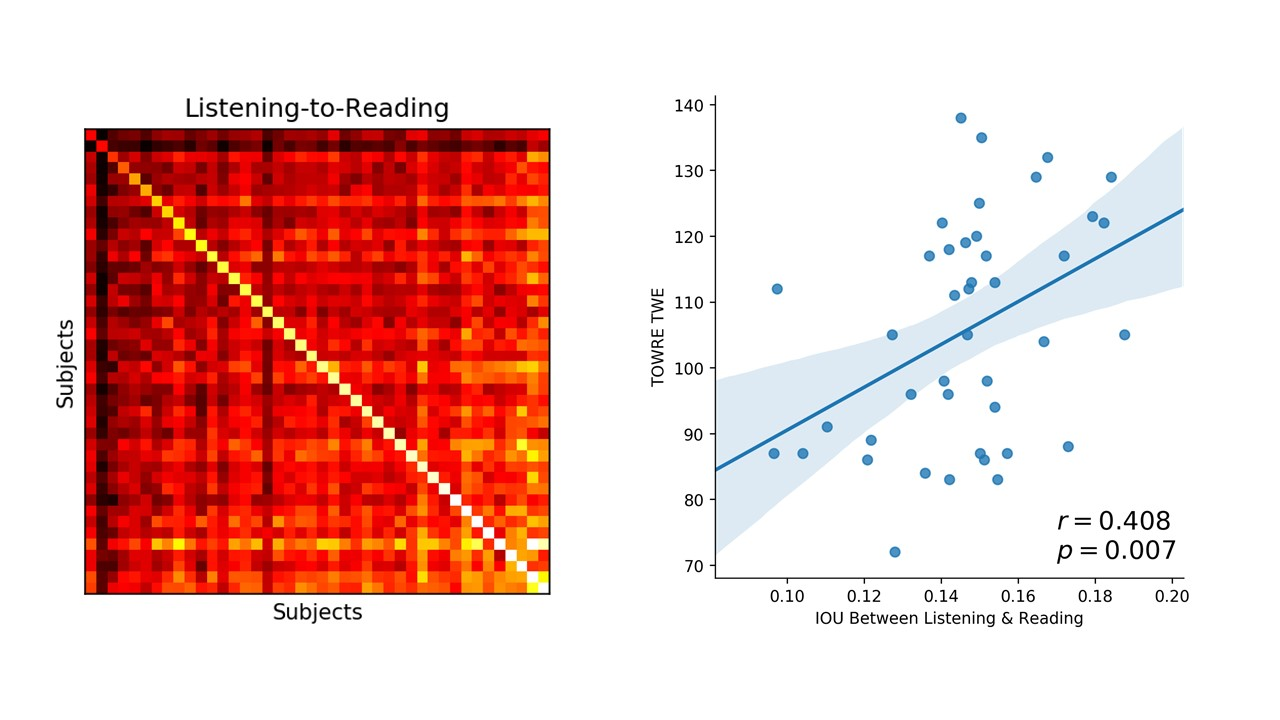
\includegraphics[width=6in]{ch4-listening-to-reading-similarity-skill}
    \caption[Network similarity between listening and reading predicts word efficiency]{Network similarity between listening and reading predicts word efficiency. We compared the listening-evoked network to the reading-evoked networks within each subject and found that it, too, correlated with reading skill.}
	\label{fig:ch4-modality-similarity-to-reading}
\end{figure}

% extended this question to encompass multiple task conditions: would individuals who are better readers have higher similarity between multiple tasks?
We next compared the similarity across all network arrays to determine the degree of variability in architecture within each subject. For each person, we created a similarity matrix describing the shared connections between each of these conditions. Then, we calculated the mean of the shared connections. Figure \ref{fig:ch4-rsn-mean-similarity} shows the distribution of within-subject IOU values across all conditions for each RSN. The global similarity was 0.364, while the highest similarities were among the visual, dorsal attention and memory retrieval conditions; the lowest were in the auditory, ventral attention, subcortical and somatomotor (mouth) regions.

\begin{figure}[t!]
	\centering
	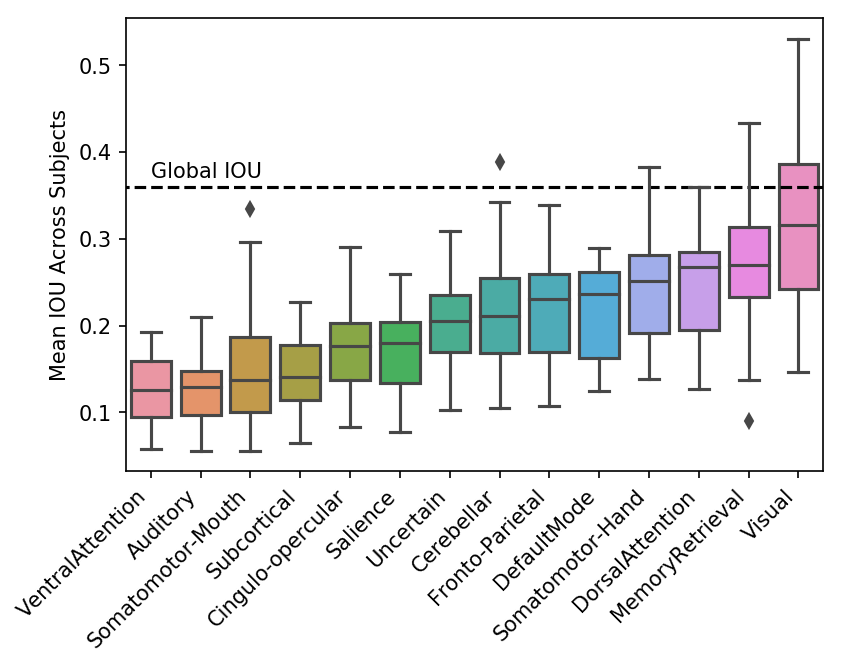
\includegraphics[height=4in]{ch4-rsn-mean-similarity}
    \caption[RSNs share a large degree of similarity]{RSNs share a large degree of similarity. At the global level, the mean similarity among task-evoked networks was higher (0.362) than any individual RSN. Several of the language- and task-oriented RSNs had very low similarity (ventral attention, auditory, somatomotor).}
	\label{fig:ch4-rsn-mean-similarity}
\end{figure}

We next correlated these measures with TOWRE scores. The mean within-subject IOU for the entire connectome (264 nodes) was significantly correlated with the TOWRE Total Word Efficiency standard score ($r = 0.324$, $p = 0.033$). Individual RSNs generally followed this trend, although a few had higher correlations: the ventral attention ($r=0.384$), fronto-parietal ($r=0.370$), salience ($r=0.352$) and default mode ($r=0.346$) networks were slightly greater than the whole-brain IOU. To test whether this was specific to reading skill or more general, we performed the same correlation using the Vocabulary scores from the WASI intelligence test. We found an even stronger correlation between global similarity measures and vocabulary scores ($r = 0.481$, $p < 0.001$), with the trend continuing for the other RSNs. 

\begin{table}[t!]
	\renewcommand{\tabcolsep}{0.09cm}
	\centering
	\begin{tabular}{lll}
\toprule
Resting-State Network & $r_{TOWRE}$ & $r_{WASI-Vocabulary}$ \\
\midrule
Global           & 0.324* & 0.481** \\
VentralAttention  &        0.384* &       0.453** \\
Fronto-Parietal   &        0.370* &       0.498** \\
Salience          &        0.352* &       0.416** \\
DefaultMode       &        0.346* &       0.509** \\
Subcortical       &        0.327* &       0.325*  \\
Somatomotor-Mouth &        0.322* &       0.402** \\
Visual            &        0.316* &       0.456** \\
Cingulo-opercular &        0.307* &       0.271   \\
Auditory          &        0.283 &       0.417**  \\
MemoryRetrieval   &        0.277 &       0.469**  \\
Cerebellar        &        0.267 &       0.346*   \\
DorsalAttention   &        0.261 &       0.464**  \\
Uncertain         &        0.136 &       0.234    \\
Somatomotor-Hand  &        0.119 &       0.285    \\
\bottomrule
\end{tabular}
	\caption[Correlation values between shared connectivity and cognitive skill]{Correlation values between shared connectivity and cognitive skills. Individual RSNs generally followed the global trend, with the exception of the unclassifiable and somatomotor (hand) RSNs.}
	\label{table:ch4-rsn-similarity-to-reading}
\end{table}

\section{Discussion}

% Recap study rationale and results
This study addressed two questions: how does task-evoked network architecture vary between two highly similar tasks, and how do individual differences in this variability relate to cognitive skills? We covered differences between reading and listening at the level of activitation, global network measures and network similarity. At all levels, we found a high degree of similarity between listening and reading relative to the other conditions, but with reading eliciting more more integration across RSNs and more variability between subjects. We found that the degree of similarity between listening and reading task-evoked networks was related to reading skill; the degree of similarity between all of the conditions, in fact, was related to reading skill. The results provide further support that variability in network architecture is not associated with increased cognitive performance. Rather, it seems to be the case that the ``evoked'' networks approximate a baseline architecture that is suprisingly stable across task demands.

% Modality differences: activation
Reading and listening elicited a similar activation profile with many overlapping areas. This is consistent with previous research and theoretical models suggesting that, after the act of word recognition, reading and listening share a common supramodal core set of processing areas \citep{Rueckl2015, Hoover1990, Price2012}. However, there were some important differences. The first was the finding of greater activity during reading along several shared language-related areas, including the temporo-parietal junction and inferior frontal gyrus. The greater activation here likely represents more effortful processing: in developing readers, there is an elevated BOLD signal for reading compared to listening \citep{Berl2011}. This elevation is also true for individuals with dyslexia who will sometime exhibit greater activation in reading-related areas compared to typically developing children \citep{Pugh2000}. 

% Dorsal attention network
The other meaningful difference is the deactivation of the dorsal attention network during reading, relative to listening. The dorsal attention network has a push-pull relationship with the ventral attention and salience networks. Because the ventral attention network is so heavily engaged during reading (viz. Chapter 3), it is likely that this reduction in DAN activity is a response to it. The DAN is closely connected to language areas including the visual word form area \citep{Bouhali2014}, but also plays a major role in guiding top-down attention, and is closely related to other executive RSNs such as the fronto-parietal \citep{Vogel2014}. Vogel and colleagues found that reading ability in typical children and adults (including decoding and passage comprehension ability) predicted increased correlations between the visual word form area and the DAN \citep{Vogel2012a}. That the deactivation of the DAN (and activation of the VAN) are present in a contrast of the two skills suggests that these attention processes are unique to reading and not general to language comprehension. To our knowledge, this is the first report of this.

% Significance of graph theory results - greater integration globally driven by visual ``de-clustering''

% Higher similarity among listening networks
Speech comprehension is ``natural'', in the sense that most everyone learns to understand language regardless of their educational environment. The greater similarity values observed when comparing the listening-evoked networks across participants may reflect the more practiced nature of speech. On the other hand, the greater variability in the reading-evoked network might be indicative of the additional interactions necessary in reading: guided control of eye movements, visual processing, additional engagement of the attention systems \citep{Mattingly1971}. There are also differences in what is encoded in speech and text.  Speech contains overt clues about the speaker, such as tone and prosody, and these can convey additional non-linguistic meaning for the listener. Reading could be considered a more purely linguistic act. Reading may thus allow more room for self-generated situation models and more independent direction of thought. 

% Relationship with similarity
As readers become more experienced, the expectation is that the task-evoked network architecture for reading would become more similar to that of the intrinsic listening comprehension system. It is thus expected that greater overlap between the two systems would be correlated with reading skill, as it was. Once again, each individual RSN was broadly representative of the global trend, but there were a few of particular note. Similarity of structure in the fronto-parietal and default mode networks were the only RSNs that outperformed the global IOU in both correlations with cognitive skills. It could be argued that these two represent the two core higher-order RSNs. High similarity in both implies that they are anti-correlated, once again touching upon the segregation hypothesis. The two RSNs that had no correlation with either measure were the ``uncertain'' nodes -- nodes whose connectivity profiles were too variable to assign to an RSN -- and the somatomotor (hand) RSN, whose connectivity may have been strongly influenced by the tapping task throughout the scans. 

%
The overarching result is that variability in task-evoked network architecture, whether it is between language tasks, simple sensory tasks or resting state, is anti-correlated with cognitive performance. Although alterations to the intrinsic organization are inevitable when performing a task, the degree of reorganization appears to be related to the task difficulty -- or at least the extent of cognitive functions employed -- with reading representing the most taxing model investigated by us. We have also seen that differences in the network architecture are robust within individuals: the correlations with reading have held across a number of different network measures. But how and when do they change? Does the relationship with reading hold true throughout the lifespan? We tackle this question in the next chapter. 
\chapter{Reading network interactions throughout development}

\epigraph{Development...}{Stanislas Dahaene}


There were two primary motivations in this study:

In the previous chapter, we established that reading does not appear to be ``simply'' a change in sensory systems. There are also more global changes in the degree of integration of different RSNs, especially those related to attention and executive control. However, this analysis was conducted in emerging readers: the participants were approximately 10 years old and were at a point in their education where basic skills were in place, but they were still relatively inexperienced readers.

It could be that the differences between the modalities were due to active support processes that were occuring between executive and attention regions, as the participants performed reading, a relatively novel task. On the one hand, advocates of a ``parallel'' model might assert that additional cognitive processes are used to ``bootstrap'' reading skill at early ages, so that differences between the two systems should decrease with maturity and reading experience as the two systems merge. On the other hand, the ``parasitic'' model of reading would predict that differences would persist, or even become exaggerated, as the two systems become more efficient for their respective tasks. In this chapter, then, we seek to replicate these results in a new cohort of subjects with a different set of passages, and then to investigate the effects of developmental maturity on the reorganizaton of brain networks during reading and listening.


\begin{itemize}
	\item Which areas ``converge'' and ``diverge'' throughout development?
	\item What shifts in connectivity patterns do we see?
\end{itemize} 

\subsection{Participants}

To collect subjects at different stages in development, participants in this study were drawn from multiple study and age groups. They fell into three categories:

\begin{itemize}
	\item A group of children (ages 8 to 10) were selected from the third wave of the longitudinal study described in chapter 2. 
	\item A group of adolescents (ages 11 to 14) were selected. These participants were part of a large, cross-sectional study on the cognitive components of reading.
	\item A group of adults (ages 18 to 30) were selected, largely from a population of university research assistants and graduate students.
\end{itemize}

All subjects provided approval and were compensated according to our IRB.

\begin{table}[t]
	\renewcommand{\tabcolsep}{0.09cm}
	\centering
	\begin{tabular}{lc}
\toprule
Measure &               Value \\
\midrule
Subjects                        &              42 \\
Mean age                        &    10.51 (0.33) \\
Sex                             &      21 M, 23 F \\
WASI Full-Scale IQ, Vocabulary  &    52.91 (9.38) \\
Test of Word Reading Efficiency &  104.66 (18.07) \\
\bottomrule
\end{tabular}
	\caption{Participant demographics for study 2.}
	\label{table:ch4-participants}
\end{table}

% \begin{figure}[t]
% 	\centering
%     \caption[Relationship between activation in visual word form area and age.]{}
% \end{figure}

% \begin{figure}[t]
% 	\centering
%     \caption[Global participation coefficient as a function of age.]{}
% \end{figure}

\subsection{Functional MRI task design}

The task design for this study paralleled that of Chapter 2. Subjects were presented up to four separate runs of a passage comprehension task. The task included two passage blocks ("PASS"), two baseline attention blocks ("ATTN") and a trailing resting-state block ("REST"). Each task was performed in either the visual or auditory modality.

The contents of the passages differed from those of the tasks discussed in chapter 2, although they were also balanced to the same third-grade reading level using Coh-Metrix. 

\subsection{Data acquisition and processing}

Functional MRI data were acquired on a Philips Achieva 3T MR scanner under the previously described parameters. Data were pre-processed in FSL and the CONN Toolbox before being analyzed. See the Methods section of Chapter 2 for a detailed description of preprocessing routines and their parameters.

\subsection{Activation analyses}

We calculated subject-level contrast maps as described previously ("listening + reading vs. rest", "listening vs. reading"). At the group-level, we used age at scan as a continuous variable to estimate the effect of age on comprehensino-related activation and modality differences.

As before, we also investigated these effects in the connectome space as well 
\chapter{Review and Summary}

A connectomics approach to reading illuminates -- not displaces -- previous neuroimaging research, much of which focused on localizing specific cognitive processes. Here, we asked how network architecture could inform our understanding of cognitive felxibility, especially in an integrative model such as reading. 

In Chapter 1, we established that reading utilizes a variety of cognitive skills whose neural substrates are distributed throughout the brain. Graph theory has enabled anlysis...
Important properties... modules... hubs...
Individual differences not well understood...
Development through interactive specialization...

In Chapter 2, we analyzed the brain at rest in developing readers. We established a basis for our specific measures... tested different thresholds... next we compared modularity to individual differences...

In Chapter 3, we observed task-evoked changes to network architecture in reading... We found that reading increased measures of integration across the brain: decreased modularity, increased participation coefficient, etc... we also found that, even during reading, there was a strong correlation between modularity and reading skill, suggesting that ``flexibility'' was built on a strong core.

In Chapter 4, we addressed the question of variability in network architecture head-on by investigating two related processes - reading and listening - and comparing them to more simple, sensory-laden attention tasks and rest. We found that there was a common core of areas activated in listening and reading, and that there was also a common network backbone. More similarity in the two language conditions was indicative of better reading. But more similarity among the other conditions was also indicative... suggesting that stability among networks is actually the more important thing...

In Chapter 5, we replicated these findings with an independent task and also described the findings across development. We found that similarity between listening and reading - and indeed, all tasks -- changed over time. ...

\begin{table}[t]
	\renewcommand{\tabcolsep}{0.09cm}
	\centering
	\begin{tabular}{c|p{10cm}}
\toprule 
Figure & Key Finding \\ 
\midrule 
\ref{fig:ch2-global-glm-covariates-thresh} & Global modularity was the graph theory measurement most predictive of reading skill. \\ 
 \ref{fig:ch2-rsn-node-modularity-corr} & Modularity in the auditory and cingulo-opercular networks was anti-correlated with reading skill.	\\ 
\ref{fig:ch3-reading-connectome-activations} & Reading comprehension induces system-level increases in the ventral attention, visual, somatomotor (mouth) and default mode networks.	 \\ 
\ref{fig:ch3-comprehension-reorganization}  & Reading is especially characterized by decreased connectivity \textit{within} sensory, dorsal attention and default mode and increased connectivity \textit{between} many different RSNs.  \\ 
\ref{fig:ch3-modularity-reading-by-condition}  & The positive relationship between network modularity and reading persists during reading comprehension.  \\ 
\ref{fig:ch4-modality-graph-theory}  & Reading comprehension requires more more integration across networks than listening. \\ 
\ref{fig:ch4-modality-similarity-to-reading} & Better readers have greater similarity between their listening and reading networks.
\bottomrule 
\end{tabular}
	\caption[Key findings.]{Key findings in Studies 1 through 4.}
	\label{table:ch6-key-findings}
\end{table}

Overall, we have sought to use reading skill as a model for how individual differences in network architecture form a basis for individual differences in cognitive processing. We have combined inferences from several different methodological approaches, including task-based univariate activation analyses, resting-state network analysis, and the combination of the two. We believe we have made a contribution to our understanding... However, there is much left to be investigated. Below, we outline a few of these directions.

\section{Individualized parcellations}

A caveat with connectomics analyses, including those presented here, are that results for the modularity analyses are often based on RSN parcellations from previous literature \citep{Power2011}. It is possible that in this sample of children, there were differences in network organization that resulted in a lower global modularity but were in fact due to differences in organization (e.g. multiple sub-modules of the default mode network). 


\section{Dynamic modeling of network architecture}

We could use dynamic modeling....




\section{Multi-modal investigations}


% Ventral attention network

\section{Conclusions}




%% Read in nomenclature
\nomenclature{DWI}{Diffusion-weighted magnetic resonance imaging}
\nomenclature{fMRI}{Functional magnetic resonance imaging}
\nomenclature{MRI}{Magnetic resonance imaging}
\nomenclature{RS}{Resting state}
\nomenclature{ROI}{Region of interest}
\nomenclature{GLM}{Generalized linear model}

\nomenclature{RSN}{Resting-state network}
\nomenclature{FPN}{Fronto-parietal network}
\nomenclature{CON}{Cingulo-opercular network}
\nomenclature{DAN}{Dorsal attention network}
\nomenclature{VAN}{Ventral attention network}
\nomenclature{DMN}{Default mode network}
\nomenclature{VIS}{Visual network}
\nomenclature{SUB}{Subcortical network}
\nomenclature{AUD}{Auditory network}
\nomenclature{SOH}{Somato-motor (hand) network}
\nomenclature{SOM}{Somato-motor (mouth) network}
\nomenclature{MEM}{Memory retrieval network}






\singlespacing
\bibliographystyle{apalike}
\bibliography{mendeley.bib}
\end{document}